%File: formatting-instructions-latex-2023.tex
%release 2023.0
\documentclass[letterpaper]{article} % DO NOT CHANGE THIS
\usepackage{aaai23}  % DO NOT CHANGE THIS
\usepackage{times}  % DO NOT CHANGE THIS
\usepackage{helvet}  % DO NOT CHANGE THIS
\usepackage{courier}  % DO NOT CHANGE THIS
\usepackage[hyphens]{url}  % DO NOT CHANGE THIS
\usepackage{graphicx} % DO NOT CHANGE THIS
\urlstyle{rm} % DO NOT CHANGE THIS
\def\UrlFont{\rm}  % DO NOT CHANGE THIS
\usepackage{natbib}  % DO NOT CHANGE THIS AND DO NOT ADD ANY OPTIONS TO IT
\usepackage{caption} % DO NOT CHANGE THIS AND DO NOT ADD ANY OPTIONS TO IT
\frenchspacing  % DO NOT CHANGE THIS
\setlength{\pdfpagewidth}{8.5in}  % DO NOT CHANGE THIS
\setlength{\pdfpageheight}{11in}  % DO NOT CHANGE THIS
%
% These are recommended to typeset algorithms but not required. See the subsubsection on algorithms. Remove them if you don't have algorithms in your paper.
\usepackage{algorithm}
\usepackage{algorithmic}

%
% These are are recommended to typeset listings but not required. See the subsubsection on listing. Remove this block if you don't have listings in your paper.
\usepackage{newfloat}
\usepackage{listings}
\DeclareCaptionStyle{ruled}{labelfont=normalfont,labelsep=colon,strut=off} % DO NOT CHANGE THIS
\lstset{%
	basicstyle={\footnotesize\ttfamily},% footnotesize acceptable for monospace
	numbers=left,numberstyle=\footnotesize,xleftmargin=2em,% show line numbers, remove this entire line if you don't want the numbers.
	aboveskip=0pt,belowskip=0pt,%
	showstringspaces=false,tabsize=2,breaklines=true}
\floatstyle{ruled}
\newfloat{listing}{tb}{lst}{}
\floatname{listing}{Listing}
%
% Keep the \pdfinfo as shown here. There's no need
% for you to add the /Title and /Author tags.
\pdfinfo{
/TemplateVersion (2023.1)
}
% These are recommended to typeset algorithms but not required. See the subsubsection on algorithms. Remove them if you don't have algorithms in your paper.
\usepackage{algorithm}
\usepackage{algorithmic}

%
% These are are recommended to typeset listings but not required. See the subsubsection on listing. Remove this block if you don't have listings in your paper.
\usepackage{newfloat}
\usepackage{listings}
\usepackage{comment}
\usepackage{mathtools}
\usepackage{subcaption}
\usepackage{multirow}
\DeclarePairedDelimiter{\ceil}{\lceil}{\rceil}
\DeclarePairedDelimiter{\floor}{\lfloor}{\rfloor}

%\PassOptionsToPackage{hyphens}{url}\usepackage{hyperref}
\usepackage{xurl}
\usepackage{float}
\usepackage[shortlabels]{enumitem}
\setlist[enumerate]{nosep}
\setlist{nolistsep,leftmargin=2.0mm}
%% Using belowskip=-3pt will cause caption to overlap tables
%\captionsetup{font=small, belowskip=-0.0pt, aboveskip=-0pt}
%\usepackage[font={bf,footnotesize},labelsep=colon, belowskip=-0pt, aboveskip=0.1pt]{caption}
\setlength{\skip\footins}{5pt}

% %% Tricks to squeeze space from section headings
%\usepackage[small,compact]{titlesec}
% \usepackage{titlesec}
% \titlespacing\section{0pt}{6pt plus 0pt minus 2pt}{0pt plus 0pt minus 2pt}
% \titlespacing\subsection{0pt}{3pt plus 0pt minus 2pt}{0pt plus 0pt minus 2pt}
% \titlespacing\subsubsection{0pt}{2pt plus 0pt minus 2pt}{0pt plus 0pt minus 2pt}
\usepackage{amsfonts}
\usepackage{xpatch}

\setlength{\textfloatsep}{0.1cm}
\setlength{\floatsep}{0.1cm}
\setlength{\intextsep}{0.1cm}
\setlength{\parindent}{0in}
%\setlength{\intextsep}{0pt plus 2pt}
%\setlength{\belowcaptionskip}{-5pt}

\begin{comment}
\xapptocmd\footnotesize{%
 \abovedisplayskip=1pt plus 0pt minus 2pt
 \abovedisplayshortskip=-1pt plus 0pt minus 2pt
 \belowdisplayskip=1pt plus 0pt minus 3pt
 \belowdisplayshortskip=1pt plus 0pt minus 1pt
 \belowcaptionskip=0pt plus 0pt minus 10pt
}{}{}
\end{comment}

\setlength{\abovedisplayskip}{0pt}
\setlength{\belowdisplayskip}{-2pt}

\newcommand{\name}{{\sc{approxEDA }}}
\newcommand{\blink}{{\sc{BlinkDB }}}
\newcommand{\greedy}{{\sc{ciGreedy }}}

% Replace below with iffalse for final version
\iftrue
%\iffalse

\newcommand{\tong}[1]{{\color{blue}{\small{\bf [Tong: #1]}}}}

\newcommand{\sm}[1]{{\color{brown}{\small{\bf [Subrata: #1]}}}}

\newcommand{\sg}[1]{{\color{purple}{\small{\bf [Shaddy: #1]}}}}

\else

\newcommand{\tong}[1]{}

\newcommand{\sm}[1]{}

\newcommand{\sg}[1]{}

\fi


\lstset{%
	basicstyle={\footnotesize\ttfamily},% footnotesize acceptable for monospace
	numbers=left,numberstyle=\footnotesize,xleftmargin=2em,% show line numbers, remove this entire line if you don't want the numbers.
	aboveskip=0pt,belowskip=0pt,%
	showstringspaces=false,tabsize=2,breaklines=true}
\floatstyle{ruled}
\newfloat{listing}{tb}{lst}{}
\floatname{listing}{Listing}
%
%\nocopyright
%
% PDF Info Is REQUIRED.
% For /Title, write your title in Mixed Case.
% Don't use accents or commands. Retain the parentheses.
% For /Author, add all authors within the parentheses,
% separated by commas. No accents, special characters
% or commands are allowed.
% Keep the /TemplateVersion tag as is


% DISALLOWED PACKAGES
% \usepackage{authblk} -- This package is specifically forbidden
% \usepackage{balance} -- This package is specifically forbidden
% \usepackage{color (if used in text)
% \usepackage{CJK} -- This package is specifically forbidden
% \usepackage{float} -- This package is specifically forbidden
% \usepackage{flushend} -- This package is specifically forbidden
% \usepackage{fontenc} -- This package is specifically forbidden
% \usepackage{fullpage} -- This package is specifically forbidden
% \usepackage{geometry} -- This package is specifically forbidden
% \usepackage{grffile} -- This package is specifically forbidden
% \usepackage{hyperref} -- This package is specifically forbidden
% \usepackage{navigator} -- This package is specifically forbidden
% (or any other package that embeds links such as navigator or hyperref)
% \indentfirst} -- This package is specifically forbidden
% \layout} -- This package is specifically forbidden
% \multicol} -- This package is specifically forbidden
% \nameref} -- This package is specifically forbidden
% \usepackage{savetrees} -- This package is specifically forbidden
% \usepackage{setspace} -- This package is specifically forbidden
% \usepackage{stfloats} -- This package is specifically forbidden
% \usepackage{tabu} -- This package is specifically forbidden
% \usepackage{titlesec} -- This package is specifically forbidden
% \usepackage{tocbibind} -- This package is specifically forbidden
% \usepackage{ulem} -- This package is specifically forbidden
% \usepackage{wrapfig} -- This package is specifically forbidden
% DISALLOWED COMMANDS
% \nocopyright -- Your paper will not be published if you use this command
% \addtolength -- This command may not be used
% \balance -- This command may not be used
% \baselinestretch -- Your paper will not be published if you use this command
% \clearpage -- No page breaks of any kind may be used for the final version of your paper
% \columnsep -- This command may not be used
% \newpage -- No page breaks of any kind may be used for the final version of your paper
% \pagebreak -- No page breaks of any kind may be used for the final version of your paperr
% \pagestyle -- This command may not be used
% \tiny -- This is not an acceptable font size.
% \vspace{- -- No negative value may be used in proximity of a caption, figure, table, section, subsection, subsubsection, or reference
% \vskip{- -- No negative value may be used to alter spacing above or below a caption, figure, table, section, subsection, subsubsection, or reference

\setcounter{secnumdepth}{3} %May be changed to 1 or 2 if section numbers are desired.

% The file aaai22.sty is the style file for AAAI Press
% proceedings, working notes, and technical reports.
%

% Title

% Your title must be in mixed case, not sentence case.
% That means all verbs (including short verbs like be, is, using,and go),
% nouns, adverbs, adjectives should be capitalized, including both words in hyphenated terms, while
% articles, conjunctions, and prepositions are lower case unless they
% directly follow a colon or long dash
%\title{Approximating Interactive Data Exploration with Reinforcement Learning %\tong{how about Approximating Interactive Data Exploration via Intent-Aware Reinforcement Learning}}

% For Page numbers
\thispagestyle{plain}
\pagestyle{plain}

\title{Reinforced Approximate Exploratory Data Analysis}
\author {
    % Authors
    Shaddy Garg\textsuperscript{\rm 1},
    Subrata Mitra\textsuperscript{\rm 1}\thanks{Corresponding Author},
    Tong Yu\textsuperscript{\rm 1},\\
    Yash Gadhia\textsuperscript{\rm 2}\thanks{Work done while at Adobe Research},
    Arjun Kashettiwar \textsuperscript{\rm 2}
}
\affiliations {
    % Affiliations
    \textsuperscript{\rm 1} Adobe Research\\
    \textsuperscript{\rm 2} Indian Institute of Technology, Bombay\\
    % shadgarg@adobe.com, subrata.mitra@adobe.com,	tyu@adobe.com\\
    % gadhiayash@gmail.com, arjun.kashettiwar@gmail.com
}


% REMOVE THIS: bibentry
% % This is only needed to show inline citations in the guidelines document. You should not need it and can safely delete it.
% \usepackage{bibentry}
% % END REMOVE bibentry

\begin{document}

\maketitle



\begin{abstract}

Exploratory data analytics (EDA) is a sequential decision making process where analysts choose subsequent queries that might lead to some interesting insights based on the previous queries and corresponding results.
Data processing systems often execute the queries on samples to produce results with low latency. 
%To make interactions faster, several recent papers proposed use of samples to reduce the query latency. %
%However sampling creates approximation errors and can mislead the users in an interactive data exploration flow. This is because the results of the previous query can get distorted due to sampling and may prompt the user to a false path of analysis, which would have been useless if the original data was used. 
%There are several sampling techniques available. 
Different downsampling strategy preserves different statistics of the data and have different magnitude of latency reductions. The optimum choice of sampling strategy often depends on the particular context of the analysis flow and the hidden intent of the analyst. 
%
In this paper, we are the first to consider the impact of sampling in interactive data exploration settings as they introduce approximation errors. We propose a Deep Reinforcement Learning (DRL) based framework which can optimize the sample selection in order to keep the analysis and insight generation flow intact. 
%To model the user behavior with implicit intents in EDA, we further propose a novel intent-aware reward function to achieve more sample-efficient DRL.
Evaluations with 3 real datasets show that our technique can preserve the original insight generation flow while improving the interaction latency, compared to baseline methods.

\end{abstract}
\section{Introduction}

%Exploratory data analytics (EDA) is a technique where analysts or data scientists attempt to understand the inherent characteristics of data and get interesting insights.
%from a new dataset or an existing dataset that is periodically being updated.
Exploratory data analysis (EDA) is an interactive and sequential process of data understanding and insight generation where a user (e.g. a data analyst) issues an analysis action (i.e. a query) against a tabular data, receives some answers, subsection of the tabular data or some visualization and then decides which queries to issue next in order to understand the hidden characteristics of the data and associated insights better~\cite{ma2021metainsight, atena2020sigmod, edasim2018kdd}.
Characteristics and insights obtained using EDA are crucial for subsequent decision making in various domains~\cite{ma2021metainsight}.
%
\begin{comment}
\noindent\textbf{Intent.}
Each of the EDA sessions corresponding to a sequence of interactions with the data, has an underlying \textit{intent} that often remains implicit to even the user until they arrive at some interesting characteristics and then follow some intuitions to find an insight.
For example: an analyst started exploring flights arrival/departure related data, noticed unusually high delay in a month for some airline and then focused to understand the root-cause. Another example: an analyst started exploring number of airlines operating from different airports and their delay patterns. But ultimately arrived at some insight about which two pair of airlines have worse connecting flight timing coordination. 
Note: none of these intents are known apriori and also does not get explicitly labeled afterwards.  
\end{comment}
%
The \textit{success} of an EDA session and the quality of insights obtained from it large depend on two things: (1) how interactive the system is (i.e. how quickly results are obtained) and (2) whether the outcome of previous sequence of queries are reliable and representative enough for an expert analyst to issue subsequent queries so as to uncover interesting characteristics. 
%
\begin{comment}
%
Several studies have shown that high interaction latency can drastically degrades the quality of insights due to mental fatigue and loss of continuity in the mental thought process~\cite{liu2014effects, moritz2017trust}. 
\end{comment}
%
\begin{figure}[t]
\begin{center}
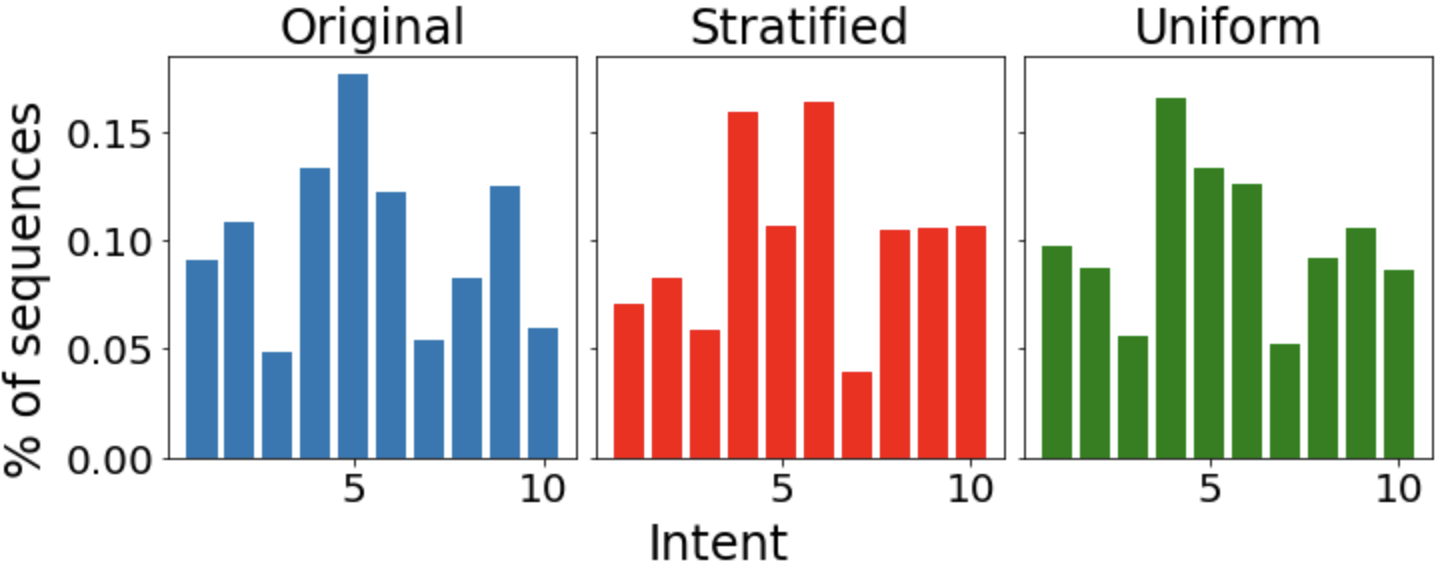
\includegraphics[width=0.85\columnwidth, height=0.25\columnwidth]{LaTeX/figures/intent_skew.png}
     \caption{Divergence of intent distribution: Single sampling strategy (stratified or uniform) for all the contexts in sequential data exploration can make user to get mislead into wrong analysis flow due to approximation errors.} 
     \label{fig:intent_skew}
\end{center}
\end{figure}

%Need for approximations
To improve latency of interactions, downsampling the data has been proposed in various works target ting approximate query processing (AQP)~\cite{chaudhuri2017approximate, park2018verdictdb, sheoran2022aaai} and visualizations~\cite{park2016visualization, moritz2017trust, porwal2022sigmod}. For large datasets that are often a target for EDA~\cite{galakatos2017revisiting, wang2014sample}, running queries on samples can substantially reduce the query latency.
%Transparency is a desirable property here because, burdening the user with another information about approximation error would make the already cumbersome EDA process even more complex. Studies have shown that users are poor at making their decisions based on approximation errors (CHI-2018).
However, sampling creates approximation errors and can mislead the users in an interactive data exploration flow, especially when the use, choice and degree of approximation is transparent to the user.
In this paper we are the first to explore a setting where an EDA system \textit{transparently} uses different forms of downsampling strategy on the original data to run the queries but protect the user from being mislead due to approximation error from poor choice of samples. 
%
Figure~\ref{fig:intent_skew} shows distributions of 10 user-intents extracted from several thousand of realistic EDA sequences on Flights data.
%using EDA simulator that can generate realistic analyses patterns similar expert users with various implicit intents~\cite{atena2020sigmod}.
It can be observed that if only a particular downsample strategy (e.g. stratified or uniform sampling) is used for every context in the entire sequence, the resulting intent distribution diverges from the ideal. 
% This indicates that blindly using any such samples can mislead the analysts.  
%
%as they often choose the next sequence of query based on display from the previous results. 
%
This is because the results of the previous query can get distorted due to sampling and may prompt the user to a false path of analysis, which would have been useless if the original data was used. Second, there are numerous sampling techniques available, such as uniform sampling with different sampling rates, stratified sampling of few different kinds, systematic sampling, cluster sampling, diversity sampling etc.
%
%
Each of these sampling algorithms are good at preserving some properties of the data at the cost of introducing approximation errors for other properties. 
%The best sampling method that can minimize the approximation error often depends on the particular structure of the query and the underlying data distribution. 
For a sequential and interactive data exploration workflow where multiple different types of queries are used on different subsections of the data, there is often not a single sampling strategy that wins over everything else. This is because, in a sequential interactive exploration the amount of approximation in the results or visualizations generated from the previous queries, influences the user decision on what next query to run. 
%Greedy solution that would pick the sample that produces lowest approximation error for the next query, is also infeasible.
%This is because actual approximation errors can not be calculated without running the query against each of the samples which can be prohibitively expensive for an interactive setting. 
Moreover, there is a trade-off between query latency and accuracy, when sampling is used.
Choosing a sample that gives higher approximation error (while making the query faster) can be desirable, as long as the approximation error does not mislead the user to make wrong decisions about subsequent analyses flow or alter the key takeaways.  

This brings us to the second major problem that we handle in this paper. EDA being fundamentally an open-ended and expertise-driven process to understand a new dataset, there is no explicit \emph{intent} that can be attributed to the analysis flow.
%For example: an analyst started exploring flights arrival/departure related data, noticed unusually high delay in a month for some airline and then focused to understand the root-cause. Another example: an analyst started exploring number of airlines operating from different airports and their delay patterns. But ultimately arrived at some insight about which two pair of airlines have worse connecting flight timing coordination. 
%Note: none of these intents are known apriori and also does not get explicitly labeled afterwards.  
Some recent papers looked at how to learn from EDA sequences performed by expert users in order to mimic those in a simulator to generate a sequence of queries and results on a new dataset, to help novice analysts~\cite{atena2020sigmod}.
Similarly~\cite{edasim2018kdd} provides suggestions to novice users about the next query to run based on learning from expert user sessions. 
While these works identify that exploratory analysis is not exactly random in nature and expert analysts usually follow few core implicit intents, but they do not handle how intent-aware learning can be performed in such situations. 
This lack of clear intent, as well as not having a clear measure of success or a implicit/explicit feedback at the end also makes our problem markedly distinct from other interactive settings such as task-oriented dialog systems \cite{liu2018dialogue,shi2019build}, conversational recommender systems \cite{lei2020interactive,zhang2020conversational} and interactive retrieval systems \cite{guo2018dialog}. When developing the learning agent for these systems, it is usually assumed that the users have a clear intent, from which the loss function or reward function can be naturally derived. However, in our task the users usually have implicit intent, which makes development of the reward function non-trivial. %\tong{As the first work focusing on approximate exploratory data analysis in an interactive setting, it is assumed that }
%interactions with a chat-bot on a particular task~\cite{}.
%\sm{Tong, can you please expand a bit? and add citations.}
%
%\sm{“The authors introduce a new concept of intent-divergence early on (ln 164), but however, never explain it in any detail. It remains unclear why the proposition prevents an intent-divergence of the user. If the analyst’s intent actually changes, preventing an intent divergence on the model side, seems to hinder their workflow.The manuscript does not include a discussion of the relevant problem of “intent-shift”.”}


To jointly address the above two challenges, we propose an intent-aware deep reinforcement learning (DRL) framework, \name, to enable the interactive exploratory data analysis in the presence of approximation errors. 
\begin{comment}
Specifically,
\begin{itemize}
        \item We down-sample the data at each time and optimize the down-sampling strategies over time, by modeling the strategies as actions in reinforcement learning.
        \item We develop a novel reward function via topic modelling to discover the user intention without labeled intention data.
        \item We develop a termination criteria to guide the model training in the sequential data exploration,
        by capturing key takeaway insights.
        This leads to more  sample-efficient intent-aware reinforcement learning.
\end{itemize}
\end{comment}
%
In this paper, we focus on how to prevent intent-divergence (\emph{i.e.}, approximation errors misleads users to a different intent). It is assumed that there is limited \textit{intent-shift} (\emph{i.e.}, change of user's core intent characteristics) in the problem setting. 
%While in this paper we are the first to address how to prevent intent-divergence (approximation errors misleads users to a different intent), 
This assumption is widely adopted in other interactive applications \cite{liu2018dialogue,guo2018dialog,tan2019drill}, although it is interesting to address the intent-shift \cite{xie2021tiage,arnold2019sector}. As the first work on approximate exploratory data analysis in the interactive setting, we leave addressing \textit{intent-shift} as future work.

\begin{comment}
subsection 1 (two datasets)
1\\
1 + 2\\
1 + 3\\
1 + 2 + 3\\

analysis:\\
subsection 2
a. different pool of down-sampling strategies to choose? corresponds to 1\\
subsection 3
b. number of cluster, 1+2+3
subsection 4
c. length of session, corresponds to 3, 1+2+3
\end{comment}

Our contributions are summarized as follows.
\begin{itemize}
    \item To our best knowledge, we are the first to identify an important yet practical problem where approximations should be used to improve interactivity in sequential exploration of data but can potentially mislead analysts to wrong analyses paths or intent-divergence. 
    \item We make a case that depending on the context of the sequential analysis, different sampling strategies would be optimal for providing lower interaction latency while protecting intent-divergence.   
    \item We novelly formulate the problem as a reinforcement learning task. Our formulation captures both the computational cost of executing the queries, as well as the sequential decisions made by users for different implicit intents. We model the choice of down-sampling strategy as the action-space and optimize the divergence of sequential interactions by an user along with the interactivity of the system, in the presence of approximations, in an intent-aware manner.
    To efficiently optimize the agent without explicit user intent, we develop a novel reward function and DRL learning stop criteria.
    \item We show the effectiveness of our technique by extensively evaluating our solution on 3 real-world datasets and against several baselines. 
    %Our method outperforms baselines in terms of intent preservation as well as latency, 
    We also present detailed ablation study and make our code and data available~\cite{open_repo}.
    
    %\item With extensive evaluations with 3 real world datasets, we show that ???...
    % \sm{Need results to be highlighted here.}
\end{itemize}

\begin{comment}
\tong{A potential flow: (please just ignore the parts which are not appropriate)
    \begin{enumerate}
        \item What is interactive exploratory data analysis? Why interactive is important.
        \item What are the challenges of developing interactive systems for exploratory data analytics? There are many existing interactive systems and applications, such as dialog system and interactive recommender system. Why developing interactive systems for exploratory data analytics is non-trival? What are the challenges?
        \begin{itemize}
            \item The computational cost is high, but the user desires real-time experience.
            \item The intent is not explicit or unclear. Thus, it is hard to develop the reward function.
            \item The intent is not explicit or unclear. Thus, it is hard to determine the termination of episode during training.
        \end{itemize}
        \item To jointly address the above challenges, we propose an intent-aware reinforcement learning framework to enable the interactive exploratory data analysis. Specifically,
        
        \begin{itemize}
        \item We downsample the data at each time and optimize the downsampling strategies over time, by modeling the strategies as actions in reinforcement learning.
        \item We develop a novel reward function via topic modelling to discover the user intention without labeled intention data.
        \item We develop a novel stop criteria to guide the model training and achieve sample-efficient reinforcement learning.
        \end{itemize}
        
        \item Our contributions are summarized as follows.
        \begin{itemize}
            \item We identify an important yet practical problem. We present the first work of ???.
            \item We novelly formulate the problem as a reinforcement learning task. To reduce the compuational cost, we model ??? as actions and optimize ??? over time. To efficiently optimize the agent without explict user intent, we devevelop a novel reward function and RL learning stop criteria.
            \item With extensive evaluations, we show that ???.
        \end{itemize}
        
    
    \end{enumerate}
}
\end{comment}



\begin{figure*}[t]
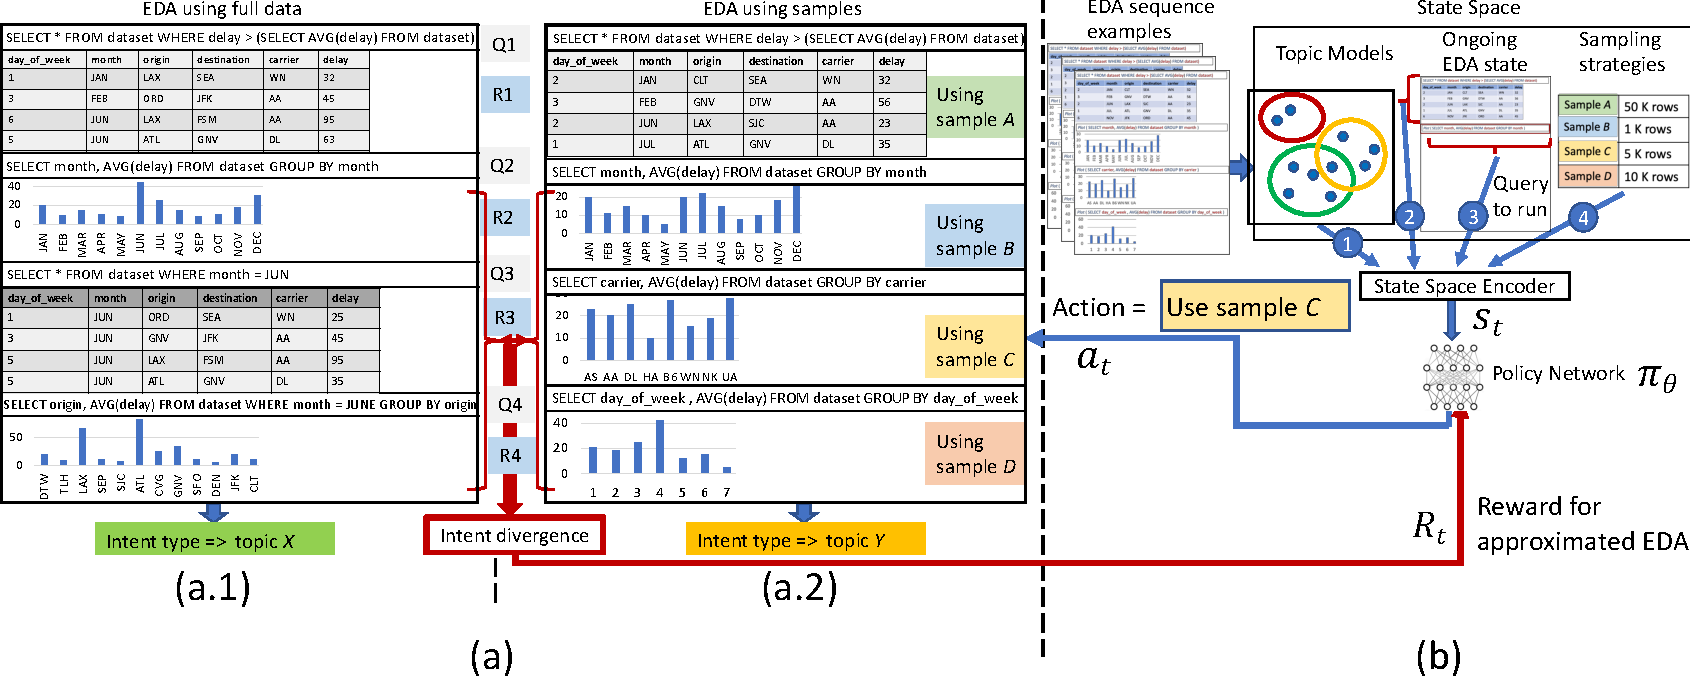
\includegraphics[width=0.98\linewidth]{LaTeX/figures/workflow.pdf}
     \caption{\textbf{(a)} Example of intent divergence between EDA sessions using full data \textbf{(a.1)} vs. using samples \textbf{(a.2)}. 
     Bad sample selection in (a.2) led to large errors in the result \textit{R2}. Consequently, user diverted from ideal query sequence and finally found misleading insight in \textit{R4}.
     \textbf{(b)} Workflow of our RL-based \name is shown. The agent transparently interacts with a live EDA session (e.g. one on the left) and chooses the best action $a_t$, i.e. the optimal sample to use for the current so that intent divergence is minimized. \name's \textit{State Space Encoder} combines 4 different information into a state $s_t$ that is used by the policy-network ($\pi_{\theta}$) to decide the best action. 
     %\tong{it seems that some content is cut in the right part of the figure 2 (b) (the state space seems to be a rectangle but the line on the very right part is missing).}
     }
     \label{fig:intent_divergence}
\vspace{-0.8em}
\end{figure*}



\section{Background and Motivations}
\begin{comment}
Exploratory data analyses (EDA) is an interactive process for insight generation for new datasets~\cite{milo2020automating, khan2020weblens, milo2018next} and low latency is important~\cite{liu2014effects},
%Several recent papers~\cite{kery2018story, rule2018exploration} present studies highlighting how computational notebooks combine code, visualizations, and text in a single document are increasingly being used by data analysts from different domains. 
%
%EDA being an interactive environment, low latency is key~\cite{liu2014effects}, and we envision that similar to the way sampling is used to speed up ad-hoc query processing in databases~\cite{park2018verdictdb}, it can also be used for EDA to run corresponding queries on samples at the back-end\cite{galakatos2017revisiting}.
%
However, EDA being a highly sequential decision making process by the data-analysts with some \textit{non-explicit intentions} in their minds, poor choice of sampling strategy in an attempt to reduce interaction latency, can completely diverge the exploration process and lead to unsuccessful EDA sessions or misleading insights.
%
\end{comment}

\subsection{Motivating Example}

%\noindent \textbf{Motivating example:}

In Figure~\ref{fig:intent_divergence}(a.1), we show example of an EDA being performed on \textit{all} the records of Flights data~\cite{Flights}. At first an analyst attempts to understand the flights delay and filters the entries that had delay higher than average (with query \texttt{Q1} and corresponding result/visualization \texttt{R1}). 
Then she wants to understand delays in detail by grouping those by \textit{month} (i.e. \texttt{Q2}) and observes from the bar-plot (\texttt{R2}) that month of \texttt{JUN} contributed highest delays.
Then she inspects by filtering the rows only for \texttt{JUN} (\texttt{Q3} and \texttt{R3}). Not finding anything obvious she groups these filtered results by \texttt{origin} airport (\texttt{Q4}) and from the result (\texttt{R4}) concludes that delays in flights originating from \texttt{LAX} and \texttt{ATL} airports is the main culprit. Then she might forward this \textit{insight} and investigate the root-cause of delays in these airports further. 
Please note: there is a lack of explicit intents~\cite{milo2020automating, ma2021metainsight} from the analysts corresponding to an EDA session.
%as they interactively decide what to do next when they see the outcome of previous results~\cite{rule2018exploration}.

Now in Figure~\ref{fig:intent_divergence}(a.2), we illustrate the problem of arbitrary sample selection if sampled are used to speed-up queries but with approximate results.
While nothing detrimental happens in the result \texttt{R1} and the analyst would still run (\texttt{Q2}) to understand the delays grouped by \texttt{month}, a poor choice of sample may not highlight the large amount of delay contributed by the month of
\texttt{JUN}. 
Therefore, not finding anything that stands out over different months, the analyst might go on to look for other anomalies or patterns of delay for different careers (\texttt{Q3} and \texttt{R3}) and further not finding anything that suspicious, attempts to understand delays over different \texttt{days\_of\_week}(\texttt{Q4} and \texttt{R4}) and concludes with a \textit{misleading insight} that delays are primarily caused of flights on \textit{$4^{th}$ day of the week}.
%
Here the analyst diverged from the ideal analysis flow (if original data was used) because of approximation errors in queries/results \texttt{Q1/R1} and \texttt{Q2/R2}. 
She finally made a wrong decisions on her choice of subsequent queries at \texttt{Q3}.   
As a result overall EDA flow diverged. 
%%Such intent-divergence can be avoided and still speed of interactions can be optimized through sampling by a more intelligent EDA-system. 

%I\noindent\textbf{Takeaway:} 
Considering the above example, appropriate sub-sample selection is crucial based on the context of EDA at each step. Thus balancing low latency for good interactive experience vs. intent and insight preservation is the goal of this paper. 
%\sm{“The authors introduce a new concept of intent-divergence early on (ln 164), but however, never explain it in any detail. It remains unclear why the proposition prevents an intent-divergence of the user. If the analyst’s intent actually changes, preventing an intent divergence on the model side, seems to hinder their workflow.The manuscript does not include a discussion of the relevant problem of “intent-shift”.”}


\subsection{Sampling Strategies}

A sample dataset $T_s$ is a subset of rows from an original dataset $T$. Following different sampling strategies select these subsets differently with different set of parameters that control the size and statistics of $T_s$.
We consider sampling strategies listed in Table~\ref{tab:actions} with different associated parameters that control the sizes of the subsamples and consequently the amount of statistical information. More details of the sampling strategies is in Appendix \textbf{\ref{app:sampling_details}}.

\begin{table}
\scalebox{0.8}{
 \begin{tabular}[ht!]{|l|l|l|}
    \hline
    {Sample Name} & {Short Name} & {Parameters} \\
    \hline
    {Uniform} & {Uni@$\tau$} & {$\tau$= [0.01, 0.05, 0.1]} \\
    \hline
    {Systematic} & {Sys@$k$} & {$k$= [100, 20, 10]}  \\
    \hline
    {Proportional stratified} & {Strat@$\tau$} & {$\tau$= [0.01, 0.05, 0.1]} \\
    \hline
    {At most $K$ stratified} & {Strat-K@$K$} & {$K$= [2k, 10k, 20k]} \\
    \hline
    {Cluster} & {Clus@$k$} & {$k$= 10, $\tau$= [0.01, 0.05, 0.1]} \\
    \hline
    {MaxMin Diversity} & {MaxMin@$k$} & {$k$= 0.1*$|T|$} \\
    \hline
    {MaxSum Diversity} & {MaxSum@$k$} & {$k$= 0.1*$|T|$} \\
    \hline
    \end{tabular}
    }
 \captionof{table}{Sampling strategies and corresponding parameters that together creates our action space. We use the \textit{Short Name} to refer these.}
 \label{tab:actions}
\end{table}

%We now provide brief background for different sampling strategies we used. 


\begin{comment}
    \item 
    \textbf{MaxMin Diversity:} 
    This maximises the minimum pairwise diversity between elements of $T_s$,
    %We define the $div$ function as follows,
    %
    %$div(T_s') = \underset{i,j \in T_s', i \neq j}{\mathrm{min}}\, d(i,j) $
    
    \item 
    \textbf{MaxSum Diversity:}
    This maximises the average pairwise diversity between elements of $T_s$. 
    %We define the $div$ function as follows,
    %
    %$div(T_s') = \frac{1}{|T_s|}\underset{i,j \in T_s', i \neq j}{\mathrm{\sum}}\, d(i,j) $
\end{comment}

\begin{comment}
\subsection{Reinforcement Learning}

In RL, at a high-level, an agent interacts with a system and tries to learn an optimized policy.
At each time step $t$, the agent observes the \textit{state} of the system $s_t$, and chooses to take an \textit{action} $a_t$ that changes the state to $s_{t+1}$ at time step $t+1$, and the agent receives a reward $r_t$.
The goal of the agent is to learn the
best policy to maximize its
expected cumulative discounted reward: $E[\sum_{t=0}^{\infty}\gamma^{t}r_t]$ where $\gamma \in (0,1)$ determines how much the future rewards contribute to the total reward~\cite{sutton1998reinforcement}.
In DRL, neural networks are used as agents to handle large state and action spaces~\cite{lillicrap2015, mnih2015human}. We explored few different RL algorithms and found that policy-gradient-based Advantage Actor Critic (A2C)~\cite{} with the neural network as a function approximator works best for our problem setup.
\end{comment}
\vspace{-0.1em}
\section{Overview of Proposed Approach}
In this paper we propose an intent-aware deep reinforcement learning (DRL)-based technique: \name{} that can make the optimal choice of samples to be used at each step of the analysis flow to speed interactions but prevents intent-divergence. 
%For example, in Figure~\ref{fig:intent_divergence}(a.2) an intelligent sample selection agent at the back-end would have decided to pick a \textit{diversified sample} (that would preserve large delay values for \texttt{JUN}) or a \textit{stratified sample} (that would include higher proportion of rows for \texttt{JUN}, if there were less number of entries in the original data). 

\begin{comment}
\subsection{Problem Formulation}
\label{sec:problem}
%
%\sm{Please review. Does this problem formulation make sense or does it becomes confusing or conflicting}

%
\tong{Is $D$ the variable $A$ in Section 4.1?}
\sm{Yes}
Let $D_0$ be the full data target for EDA.
Let $D'$ = $\{D_i\}_{i=1}^n$ be $n$ subsamples created from $D$ and $|D_i| < |D_0|$ for $i \in [1, n]$ where $|.|$ denotes size (\# of rows). 
Let an $l$ length EDA session $e=\langle \{q_j(D_i), v_j(D_i)\}_{j=1}^l | i \in [1,n]\rangle$ be comprised of an alternating sequence of queries $q_j(.)$ and corresponding results/visual output $v_j(.)$ performed on data $D_i$. 
%

Let $I$ be the set of implicit intents embedded in the distribution of all $e$, the EDA sessions.
%\sg{What is e here?}\sm{e is an EDA sequence/session}
%
Let $I^{D_0}$ be original distribution of the intents $P(I|D_0)$, i.e. when all EDA was done using full data $D_0$.
Let $I^{D'}$ be the distribution $P(I|D')$, i.e., EDA is approximated using only subsamples.
Our goal is to find optimal subsample $D_i, i \in [1,n]$ for each step of the EDA $\{q_j(.), v_j(.)\}$ such that $Div(I^{D_0}||I^{D'})$ is minimized with $I$ as the support.
%

We define $Div(I^{D_0}||I^{D'})$ as the \textbf{intent-divergence} between the EDA performed using full data and approximate EDA using only subsampled data.  \tong{if we formally define this metric, is this metric reflected in or related to some evaluation metrics in Section 5.3? If not, might it be better not to formally define this metric?}

%\sm{We should clarify intent-divergence here.}
\end{comment}


\subsection{Design of \name{}}
%\vspace{-0.2em}
We show the high-level system architecture of \name{} in Figure~\ref{fig:intent_divergence}(b).
\name{} first takes in a history of EDA sequences performed by human data analysts and uses Topic Modeling technique to identify a set of implicate intents in those sequences. 
Then the RL-agent of \name{} takes into account:
(1) these clusters of these latent intents,
(2) the history of the ongoing EDA exploration session including the query used so far and the corresponding display-outputs (graphs and dataframes),
(3) the next query the user is intending to run,
and (4) the set of available samples created with different sampling strategies along with the size of each. 
The RL-agent, which is parameterized by a deep neural network~\cite{lillicrap2015, mnih2015human}, is trained \textit{offline} to choose the optimal sampling strategy as the best \textit{action} for different context of the analyses and intent. We considered alternate RL algorithms (DQN [\cite{mnih2013playing}] and REINFORCE [\cite{sutton2018reinforcement}]) but found the convergence and stabilization of A2C training (Lillicrap et. al), which is a hybrid between value and policy based approach, was better and reduces variance.
The best action corresponding to each step, i.e. for each query in the EDA session attempts to minimize the divergence of intents due to approximation error caused by different samples, while optimizing for lower latency. 

%\tong{}

%\noindent \textbf{Why DRL?}
%In our system, we choose the optimal sampling strategy by DRL. In RL, at a high-level, an agent interacts with a system and tries to learn an optimized policy.
%In DRL, neural networks are used as agents to handle large state and action spaces~\cite{lillicrap2015, mnih2015human}.
For our problem, lack of explicit intents in the EDA sessions, a moderately large action space of possible sampling strategies combined with the choice of parameters for each of those strategies that would control the statistical information preserved in the samples and associated trade-off for latency based on the size of the samples ($\#$ of rows), makes this a complex optimization problem. 
Appendix\textbf{~\ref{app:discussion}} further discusses why RL better choice instead of greedy solutions.

\subsection{Intent Identification}
\label{sec:intent_identification}



The problem of intent aware sample selection requires us to first solve the problem of identifying the intent of the user given a query sequence $Q_j$. 
%We use the set of EDA sequences generated by a simulator~\cite{atena2020sigmod} to model different intents.
%
% \tong{we may cite some intent-ware papers without using RL.}
%
%In this section, we draw an analogy between a collection of natural language documents and a sequence of queries. A word, which is a fundamental unit of a document corresponds to a query in our case. 
Similar to analyzing natural language texts to understand the topics, we can analyze query sequences to discover the user intents. Inspired by the previous work which uses topic modeling techniques to model goals
that users carry out by executing a sequence of commands \cite{aggarwal2020goal}, we leverage topic modeling to discover the user intent, which is further used to derive the reward signal as detailed later in Section \ref{sec:reward}. 

%\sm{“They however do not properly motivate Topic Modeling as a means to identify the intent of a user; Topic Modeling appears to be an arbitrary choice and is disconnected from the actual intent of the user. Topic Modelling is a very limited modelling technique and involves many delicate choices to get right even when it is appropriate. One obvious problem in the setting at hand is how many topics to choose to match the wide (potentially infinite) range of potential user intents during their exploration.”}
%\sg{https://dl.acm.org/doi/10.1145/3383313.3412255}


Specifically, we use a bi-term model (BTM) \cite{btm2013www} for the identification of the intent. Each topic output from the BTM model corresponds to an intent. For a query sequence $Q_j$, the output from the BTM model, \(\phi\) is the probability distribution over all the topics.

{\small
\begin{equation}
    \phi(Q_j) = \{P(t=t_i | Q=Q_j)\}_{i=1}^kK
\end{equation}
}
Here $K$ is the number of topics, and each $t_i$ corresponds to a topic. To get the corresponding intent, we take the $argmax$ over the probability distribution. The obtained intent, $I_{Q_j}$ is considered to be the user intent by \name{}.

{\small
\begin{equation}
    I_{Q_j} = argmax(\{P(t=t_i | Q=Q_j)\}_{i=1}^K)
\end{equation}
}
To decide the optimum number of topics for the BTM model, we use a coherence evaluation metric, the UCI measure~\cite{newman2010evaluating}, defined as

{\small
\begin{equation}
    score_{UCI}(q_i, q_j) = \log{\frac{p(q_i, q_j)}{p(q_i)p(q_j)}},
\end{equation}
}
where $p(q_i)$ represents the probability of seeing a query $q_i$ in a query sequence and $p(q_i, q_j)$ is the probability of observing both $q_i$ and $q_j$ co-occurring in a query sequence computed as follows,$p(q_i) = \frac{M(q_i)}{M} \text{ and } p(q_i, q_j) = \frac{M(q_i, q_j)}{M}$, where $M(q_i)$ is the count of query sequences containing the query $q_i$, $M(q_i, q_j)$ is the count of sequences containing both $q_i, q_j$ and $M$ is the total number of query sequences.
The $UCI$ score for an intent $I$, is calculated as, $mean\{score_{UCI}(q_i,q_j | q_i, q_j \in I, i \neq j)\}$ and the overall UCI score the average across all intents. Higher UCI score is indicative of better grouping because one would expect two queries belonging to the same intent to show up together regularly in the query sequences. We compute the overall UCI score for all $K \in [2,15]$ and choose the best K.

% \sm{We need the plot for housing as well.}

% \sm{Please add how to you choose he optimum cluster.}
% \sm{Please explain these and the plot almost similarly as the Goal-driven paper. }

\section{RL Formulation}
%\vspace{-0.2em}

%\subsection{RL Formulation and Rewards}
We use RL for intent-aware sample selection the agent learns the optimal policy modeled as a conditional distribution $\pi(a|s)$, specifying the probability of choosing action $a \in A$ when in state $s \in S$. 
If the agent chooses an action $a \in A$ at state $s \in S$, it receives a reward $r(s,a)$.

\subsection{Action Space}
\vspace{-0.2em}
A set of $n$ samples are pre-created using different sampling strategies (and of different sizes). 
These samples are the set of $n$ actions: $A = \{a_1, a_2, .., a_i\}_{i=1}^n$ for the RL-agent.

\subsection{State Space}
%\vspace{-0.2em}
As shown in Figure~\ref{fig:intent_divergence} (b), we use 4 components while deciding which action to choose. These components form the state space of the RL agent. The agent at each timestep $t$ for a query $q_t$ has access to the ongoing EDA state comprising of the previous $k$ queries $\{q_{t-1}, q_{t-2}, ..., q_{t-k}\}$ and their result vectors $\{v_{t-1}, v_{t-2}, ..., v_{t-k}\}$. 
%\sm{What is the notation for a query? small q or capital Q? I think we are mixing it up.}
%\sg{q stands for a single query and Q stands for a sequence of queries}
Since reducing the latency is one of the primary goals of the agent, it also takes into account the latency encountered till timestep $t$. We denote this latency factor by $C_t=\sum_{i=0}^t c_i$, where $c_i$ is the latency associated with running a query $q_i$ on a sample $a_i$. Finally, to preserve the intent information of the sequence, we also include the probability distribution over all the topics, $I_t = \phi(Q_t)$ as one of the state space components. Formally, the state space can be written as, 
{\small
\begin{equation}
\label{eq:state_space}
    s_t = \{ ((q_{t}, v_{t}),(q_{t-1}, v_{t-1}), (q_{t-2},v_{t-2})), I_t, C_t  \}
\end{equation}
}

Once the agent chooses an action $a_t \in A$, the agent moves to the next state $s_{t+1}$ and returns a result (display vector) $v_t$, as the result of the query $q_t$. Our goal here is to choose $a_t$ at each step, such that the overall latency for the sequence is minimised, simultaneously preserving the intent of the generated sequence. To do this we develop several reward functions and propose an intent-aware RL framework based on A2C methodology~\cite{mnih2016asynchronous}.
Details of our training algorithm is given in supplement (\ref{app:training}).
% \sm{Citation not coming.}

\subsection{Reward Design}
\label{sec:reward}
\vspace{-0.2em}
\name{} calculates the reward at the end of each exploratory session. For the calculation of reward, we use a set of sequences generated on the original table and we refer them as ground truth, $O_i \in O$. Each $O_i$ is a sequence of queries. Similarly, the sequence generated by the agent at the end of each episode is represented as $Q_t$.
Reward design combines following components.

\noindent\textbf{Latency Reward. }
Choosing samples of smaller size gives lower latency and hence this reward is calculated as:
%At a state $s_t$, when an agent takes an action $a_t$, the total number of rows read by the agent while taking that action is termed as $|{T_s}|$ and the total number of rows in the original dataset as $|T|$. Then the immediate reward after taking an action $a_t$ is,

{\small
\begin{equation}
\label{latency_reward}
    R_{latency} = \sum_{t=1}^{l} r(s_t, a_t),
\end{equation}
}
,where $r(s_t, a_t) = 1 - \frac{|{T_s}|}{|T|}$, where $T_s$ is the time taken to run on a sample, $T$ is the time taken to run on the original dataset, and $l$ is the length of the sequence in the session. 
This reward helps to navigate the trade-off between lower approximation error vs. lower latency. 
%that the agent does not always select the sample with the most amount of data, as that data usually leads to best approximation of data but high latency.

\noindent\textbf{Intent Reward. }
Intent reward is designed to prevent divergence of EDA sequences due to approximations (\S!\ref{sec:problem}). 
%While choosing the smallest samples using the latency reward will lead to reduced waiting time for the user, but it will often lead to diverging of intent after some point. If we only use the latency reward, the agent will often choose the smallest sample out of all the available ones. 
%We not only want the RL-agent to choose samples that will minimize time, but also to preserve the intent of the analyses. 
To prevent intent-divergence we introduce two components in the intent reward. We denote the distance function for distance between two query sequences corresponding to two EDA sessions to be $Distance(Q_1, Q_2)$. We define the reward function to be,

{\small
\begin{equation}
\label{eq_eda_sim}
    R_{dis} = 1 - Distance(Q_t, Q_{ground}).
\end{equation}
}
where $Q_{ground}$ is the closest sequence to the given sequence $Q_{t}$ in the original set $O$.
 We use \texttt{EDA-Sim} defined in \cite{atena2020sigmod} as distance metric. EDA-Sim compares the content and order of the results from the query sequence to calculate a similarity score. Based on this score we find a sequence from $O$ that is closest with current sequence.
%, so that we can match our trajectory with one of the sequences from the original sequences. 

However, it is possible that two sequences may not have the exact same ordering or content (resulting in low EDA-Sim score) but still overall have same underlying intent. 
%only the above intent reward is not sufficient for preserving the intent. There are cases where query sequences with different intents may have a low EDA-Sim value. 
Hence we also use Euclidean Distance ($EuD$) to compare intent identified from topic model distributions (\S~\ref{sec:intent_identification}) as follows:


{\small
\begin{equation}
\label{topic_reward}
    R_{topic} = 1 - EuD(\phi(Q_t), \phi(Q_{ground}))
\end{equation}
}

Full intent reward is: $R_{intent} = R_{dis} + \delta*R_{topic}$.
%($\delta$ is hyperparameter),

%{\small
%\begin{equation}
%\label{intent_reward}
%    R_{intent} = R_{dis} + \delta*R_{topic}
    %_{intent} = R_{dis} + R_{topic}
%\end{equation}
%}

%The above rewards ensure that the topic distribution matches with that of the closest sequence.
\begin{comment}
\noindent\textbf{Batch Intent Reward}
When using intent and latency rewards, the agent might always select samples corresponding to a only a few intent. To ensure that the agent also learns to preserve the distribution of different intents across various EDA sessions, we enforce another reward called batch-intent-reward.
%We want our agent to choose samples, so as to preserve the original distribution of intent over ground sequences $O$. Therefore, %
We add a component of reward which is the difference in consecutive differences between intent distributions. We term this reward as,
{\small
\begin{equation}
    R_{batch} = \bigl(D(U(Q_{t-1})) - D(U(O))\bigr) - \bigl(D(U(Q_{t})) - D(U(O))\bigr),
\end{equation}
}
where $U$ is the distribution of intent over the sequences.
\end{comment}

\noindent\textbf{Termination Reward. }
While the whole EDA session, comprising of query and corresponding visualization sequences, are important to the analyst, usually last few queries are the most important as they provide key takeaway insights. 
%
%Even after, matching intent of the user with the closest sequence, it might not be enough to preserve these insights. 
%
Therefore, the another component of our reward is based on final insight preservation. The first subcomponent $R_{match} = \{0, 1\}$, a binary 
reward if the last $k$ queries of the generated sequence $Q_t$ match with at least one of the ground truth sequence belonging to the same intent cluster.
%
However, often different query sequence lead to similar insights. Therefore, the other subcomponent  $R_{recall}$ as the top-k recall for the display vectors (results) from the generated sequence, $Q_t$ and the closest sequence identified, $Q_{ground}$ in Eqn.~\ref{eq_eda_sim}.
Full termination reward is: $R_{term} = R_{match} + R_{recall}$.

%With all the reward functions, the reward function $J_R(\pi)$ is
%
%{\small
%\begin{equation}
%\label{policy_equation}
%    J_R(\pi) = \mathbb{E}_{a_t \sim \pi_\theta}[R_t],
%\end{equation}
%}

Complete reward is $R_t = R_{latency} + \beta*R_{intent}+\gamma*R_{term}$.

% is,
%{\small
%\begin{equation}
%\label{total_reward}
%    R_t = R_{latency} + \beta*R_{intent}+\gamma*R_{term}.
%\end{equation}
%}
%To train the RL model with the given reward function we use the policy-gradient bases Advantage Actor Critic (A2C) with neural network as a function approximator for the policy and value functions. 
%For the policy network and the value network, we have different neural networks, each with 2 hidden layers of latent dimension 64.
%After learning the policy $\pi_\theta(a|s_t)$ by the above reward function, the action at each step is chosen via,
%{\small
%\begin{equation}
%\label{action_argmax}
%    a_t = argmax_{a \in A}\pi_\theta(a | s_t).
%\end{equation}
%}

\begin{comment}

\subsection{Problem Formulation}

\sm{+ mention run-time sampling has significant latency and complicated to implement engineering-wise}
Our task is to choose the best sampling strategy for an interactive exploratory data analysis workflow minimising the cost of running the queries while preserving the intent of the analyst performing this analysis. We pre-compute a set of $n$ samples, $A$ for the dataset given. This is done because online sampling techniques have significant latency and are complex to implement. The agent is given this set of sampled datasets with $n$ samples, \( A = \{a_1, a_2, .., a_i\}_{i=1}^n \), \tong{?} where each $a_i$ is a downsampled version of the original dataset. The computation cost array \( C = \{c_1, c_2, .., c_i\}_{i=1}^n \), where each $c_i$ is the downsampling percentage for $a_i$. \tong{unclear whether it is a linear function, shaddy-remove} The cost of computation is directly proportional to the number of rows in a dataset and we use this to train our RL agent.
\tong{it is unclear why D is a finite set. May need some explanations.}

The agent is provided with a sequence of queries of length $l$, \(Q = \{q_1, q_2, .., q_i\}_{i=1}^l\) to be run on a dataset, $a_0$. We denote the intent of the user interacting with the query engine to be $I_{orig}$ \tong{?}. We formulate this decision problem as a Markov Decision Process (MDP) \tong{when introducing MDP, you may describe in a way similar to Section 2.1 in https://proceedings.neurips.cc/paper/2019/file/52130c418d4f02c74f74a5bc1f8020b2-Paper.pdf}. At each step $t$ in the query sequence, the state of the agent is $s_t$, and the possible action space is $\{a_i\}_{i=1}^n $. The state $s_t$ can be represented by the vector of $k=2$ previous queries and their display vectors, the intent distribution from the intent identification part of our pipeline, and the latency cost uptil that point. Formally, it can be written as
\begin{equation}
\label{eq:state_space}
    s_t = \{ ((q_{t}, v_{t}),(q_{t-1}, v_{t-1}), (q_{t-2},v_{t-2})), I_t, C_t  \}
\end{equation}
\tong{?}
Here $v_i$ represents the display vector corresponding to the query $q_i$. Detailed information about this can be found in Section~{3.3}.

Our goal here is to choose $d_t$ at each step $s_t$, such that the overall cost $C_{total} = \sum_{i=0}^l c_i$ \tong{discount?} for the sequence is minimised, simultaneously preserving the intent of the generated sequence, $I_{gen}$ \tong{?} matches the original intent, $I_{orig}$. 
\tong{We may better define `intent' and `matches the original intent' somewhere in the paper.}
Once the agents picks an action $a_t \in A$, the agent moves to the next state $s_t+1$ and returns to user $v_t$, which is the result of the query $q_t$. To solve our MDP problem \tong{optimize XX over time}, we propose an intent-aware RL framework which uses A2C algorithm with intent based reward.
\end{comment}

\begin{comment}

\subsection{Intent Modelling}
\sm{Should go before Model Overview}


\sg{
\colorbox{yellow}{Experiment section 2: } - Include heatmaps for the generated sequences showing the distrubution of the queries in different clusters. 
\begin{itemize}
    \item Try various clustering sizes (6,8,10) and see what makes sense. Maybe include all the results here.
    \item Show the diverging intents on the original and fixed sampling approach.
\end{itemize}
}

The problem of intent aware sample selection requires us to first solve the problem of identifying the intent of the user given a query sequence $Q_j$. We use the set of EDA sequences generated by the simulator to model different intents.

%We draw an analogy between a collection of natural language documents and our set of generated query sequences. In a document, a word is a fundamental unit. 
\tong{we may cite some intent-ware papers without using RL.}
Similar to analyzing natural language documents to understand the topics, we can analyze the query data to discover the user intents\cite{goal2020recsys}
A query $q_i$ is a fundamental unit for the construction of a query sequence. We use a bi-term model (BTM) \cite{btm2013www} for the identification of the intent. Each topic output from the BTM model corresponds to an intent. For a query sequence $Q_j$, the output from the BTM model, \(\phi\) is the probability distribution over all the topics.
\begin{equation}
    \phi(Q_j) = \{P(t=t_i | Q=Q_j)\}_{i=1}^k 
\end{equation}
Here $k$ is the number of topics, and each $t_i$ corresponds to the topic. For getting the intent, we take the $argmax$ over the probability distribution
\begin{equation}
    I_{Q_j} = argmax(\{P(t=t_i | Q=Q_j)\}_{i=1}^k)
\end{equation}
This $I_{Q_j}$ is considered to be the intent for our problem.

\end{comment}

\begin{comment}
\subsection{Model Overview}

\subsubsection{State-Space Encoding}
Our model takes in a query, $q_t$ from a user at time step $t$. We support three types of EDA operations ($OP = \{\tt{FILTER}, \tt{GROUP}, \tt{BACK}\}$). Each operation $o \in OP$ is defined as follows,
\begin{itemize}
    \item $\tt{FILTER(attr,op,term)}$ is used to select data tuples that match a criteria. It takes an attribute, a comparison operator (e.g. equals, contains) and a numerical/textual term, and results in a new display representing the corresponding filtered subset.
    \item $\tt{GROUP(g\_attr, agg\_func, agg\_attr)}$ is used to group and aggregate the data. It takes a single attribute to be grouped by, an aggregation function and another attribute to employ the aggregation function on.
    \item $\tt{BACK()}$ allows a backtrack to the previous display in order to enable an alternative exploration path.
\end{itemize}
This query is encoded into a six dimensional vector. The encoded query, $q_t$ can be represented as $q_t = \{o, attr, op, term, g\_attr, agg\_func\}$.
We design the state space of our model such that it can capture the history (queries and their results) of EDA session along with the intent identified, $I_t$ from the BTM model and the cost incurred $C_t$ by the agent. Figure~\ref{} illustrates different components of our state space. To preserve the broader context in which the results are generated, we concatenate last two query ($q_{t-1}, q_{t-2}$) and display vectors ($v_{t-1}, v_{t-2}$) to the current query and display vector. The state space can be thus represented as (\ref{eq:state_space}).


\subsubsection{Action Space}
At each time-step t, for the query, $q_t$, our agent outputs an action $a \in A$. Each of this action corresponds to a downsampled dataset $a_i$. Each action has a corresponding cost of running $c_i$, represented by the fraction of rows processed by the agent while taking that action. 
\sm{Notational explanation. Details on how it goes back to the EDA sequence.}

\subsubsection{Neural Network Architectures}
The A2C model has two components - an actor (policy based) and a critic (value based). The actor takes in the input and outputs the best action whereas, the critic evaluates the action by computing the value function. We model the actor (policy network) as a function approximator using a fully connected neural network. The critic (value network) is also separately modelled by a fully connected neural network. The critic receives the state and the action from the actor as its input and it outputs the Advantage value. 
The training for both the networks happen separately, using gradient descent to find the global maximum and update their weights. As time passes, the policy network tries to learn the best policy and the value network gets better at evaluating those actions.

\end{comment}
\begin{comment}
\sm{A2C -- what is A2C? How many networks, how does updates work.
For us what is the high-level architecture.}

\sm{Refer to the Figure to explain each component of state Space}
\end{comment}

% \subsection{Training Strategy}
% \sm{Give the detailed algorithm for RL using A2C showing updates.}

% \tong{This section is called model overview, but no model details (e.g., parameterization) are introduced. Please see an example in Section 3.1 of https://arxiv.org/pdf/1805.00145.pdf.}
% \sg{Explain our setup for the generation of the EDA sequences, so that we can further in the paper use it to motivate what we are trying to do. This will include the limitation that we don't have humans to generate the sequences and hence we are trying to model humans via this simulator from the ATENA paper.\\
% After this we can motivate our problem by showing some sequences from the simulator on a fixed sample and the original table and show how they lead to different insights.\\
% \colorbox{yellow}{Experiment section 1:} - Need sample sequences to motivate our introduction, we already have 1, we need 1 more. What we are trying to do here is we will show that there is a divergence in the sequence. We fix the first 3 sequences and then let the simulator run its course on the rest. We have to show the results qualitatively as shown in the demo.
% Give an overview of the solution approach.}

\noindent\textbf{Intent-divergence vs. intent-shift}
This paper addresses the problem of \textit{intent-divergence} where the users' have a set of consistent implicit objectives/intents during the EDA. 
While \name{} deliberately introduces a bias towards a set of intents inferred from historical analysis sequences, this is justified as real expert users often follow some standard exploration strategies and look for similar types of insights even on new datasets as observed by multiple prior works~\cite{atena2020sigmod, jain2016sqlshare, milo2018next} and do not perform random explorations.
However, if such implicit objectives suddenly change causing an \textit{intent-shift}, then \name{}'s current design would not be able to detect that. 
In this paper, it is assumed that there is limited \textit{intent-shift} (\emph{i.e.}, change of user's core intent characteristics). 
%While in this paper we are the first to address how to prevent intent-divergence (approximation errors misleads users to a different intent), 
This assumption is widely adopted in other interactive applications \cite{liu2018dialogue,guo2018dialog,tan2019drill}, although it is interesting to address the intent-shift \cite{xie2021tiage,arnold2019sector}. As the first work on approximate exploratory data analysis in the interactive setting, we leave addressing \textit{intent-shift} as future work.

%\vspace{-0.5em}
\subsection{Implementation \& Deployment}

\begin{algorithm}[th]
        \begin{algorithmic}[1]
        \label{alg:alg1}
        \caption{\name{}'s Training Algorithm}
        % \textbf{Input} Dataset $D$
        \STATE Train the ATENA~\S{5.2} on given dataset $D$
        \STATE Generate sequences $O$ using ATENA
        \STATE Train a $BTM$ model $\phi$ with $K$ topics on $O$
        \STATE Create sample set $A=\{a_1,a_2,...,a_i\}_{i=1}^n$
        \STATE Initialise A2C model
        \FOR{$i = 1,...,episodes$}
            \STATE Initialize the state space $s_t$ as in (\ref{eq:state_space}) with zeroes
            \FOR{$t = 1,...,l$}                    
                    \STATE Generate a query $q_t$ from the simulator
                    \STATE Take action $a_t$ for the given $s_t$
                    \STATE Update $s_t$ with latest query $q_t$, display vectors $v_t$, latency $C_t$ and current intent as $\phi(Q_t)$
            \ENDFOR
            \STATE Calculate Individual rewards using~\S{4.3}.
            \STATE Calculate the total reward $R_t$
            \STATE Calculate $J_R(\pi) = \mathbb{E}_{a_t \sim \pi_\theta}[R_t]$
            \STATE Compute loss functions $\mathbb{L}(\theta)$ for policy network
            \STATE Compute $\mathbb{L}(\omega)$ for value network
            \STATE Update A2C model
        \ENDFOR
        \end{algorithmic}
    \end{algorithm}

%\vspace{-0.2em}
Algorithm 1 explains the steps we use for training our RL Agent. It takes in the dataset $D$, processes it by creating samples as shown in line 4 and training ATENA simulator on the same as shown in line 1. Then on the generated sequences, a BTM model is trained in line 3. Once this is done, we then start the training of our agent as demonstrated in lines 5-18 of Algorithm 1. We follow episodic training where we calculate rewards at the end of each episode as shown in line 13. Once we calculate the total reward, we compute the loss functions and update both actor (policy) and critic (value) networks as explained in \S{\ref{apps:model_implementation}}. Appendix \textbf{\ref{app:discussion}} discusses deployment aspects.


%This limitation is widely applicable to other intent-based systems as well~\cite{} we leave this as a future work.
%\sm{Tong - you have any references?}\tong{Look}
%\sm{“The authors do not sufficiently discuss the downsides of an intent-aware sampling approach. For example, the proposed strategy introduces a bias towards, unlike its main competitors that sample uniformly at random. Consequently, it remains unclear whether the proposed method can estimate a truly exploratory user intent, as it will be more random (ln. 118). The introduced bias appears to be more problematic than the accumulated approximation error.”}

%\sm{“The authors introduce a new concept of intent-divergence early on (ln 164), but however, never explain it in any detail. It remains unclear why the proposition prevents an intent-divergence of the user. If the analyst’s intent actually changes, preventing an intent divergence on the model side, seems to hinder their workflow.The manuscript does not include a discussion of the relevant problem of “intent-shift”.”}


\begin{comment}
Training of this model requires us to have human generated sequences of queries on a given dataset and these sequences not readily available. So for the purpose of this paper, we are generating these query sequences using a simulator proposed by \cite{atena2020sigmod}. This simulator mimics a human expert trying to do EDA on a given data and generates sequences, $Q$ of fixed length $l$.
For each query, the EDA operations considered are \emph{Filter}, \tong{we may use \tt{Filter}} \emph{Group} and \emph{Back} where,
\begin{itemize}
    \item \emph{FILTER(col, op, term)} is used to select data tuples that match a criteria. It takes an column, a comparison operator (e.g. equals, contains) and a numerical/textual term, and results in a new display, the corresponding filtered subset.
    \item \emph{GROUP(g\_attr, agg\_func, agg\_attr)} is used to group and aggregate the data. It takes a single attribute to be grouped by, an aggregation function and another attribute to employ the aggregation function on.
    \item \emph{BACK()} allows a backtrack to the previous display in order to enable an alternative exploration path.
\end{itemize}
Each query $q_i$ of the sequence $Q$ is represented as a six dimensional vector
\begin{equation}
\begin{multlined}
    q_i = [Operation Type, Column ID, Filter Operator,\\
     Filter Term, Agg Column ID, Agg Function] 
\end{multlined}
\end{equation}
\tong{I would suggest to define notation for each of them in the above.}
Here $OperationType$ takes on values $\{0,1,2\}$, where 0 represents back, 1 represents filter and 2 represents group type query.

The set of EDA sequences, $QS = \{Q_1, Q_2, .., Q_j \}_{j=1}^m$ \tong{lower case for consistency} are generated on the original dataset $D_0$ and are considered to be the original EDA sequences which mimic a data analyst. These sequences are then fed into the intent model, which uses topic modelling to cluster these sequences into different topics. \tong{this part needs to be presented more formally. I would suggest to follow some existing papers, instead of starting from scratch.} Each of these topics corresponds to different intent. 
We then train our RL agent on these generated sequences and the identified intents using a novel reward function which takes into account the intents and the given latency, and chooses an action from the given downsampling strategies. Figure \ref{fig:model_overview} explains how our model will be used by an analyst who wants to do EDA. \sg{Add a figure for the model architecture}
\end{comment}

\begin{comment}
\sg{Include a figure for the reference of training.}

\begin{figure*}[t]
\centering
\begin{minipage}{0.5\textwidth}

\includegraphics[width=1.0\linewidth]{figures/solution_outline.png}
     \caption{Model Overview. \tong{we may use pdf or ps format for the figure (instead of png), to get a higher resolution figure? Besides, this might be 'system overview'. Intent-ware is a key point, but is downplayed in the figure for now. Where is the topic model?}}
     \label{fig:model_overview}
\end{minipage}%
\hfill
\begin{minipage}{0.5\textwidth}
\centering
%
\includegraphics[width=\linewidth]{figures/framework.png}
\caption{}
\label{fig:framework}
\end{minipage}
\end{figure*}

\end{comment}

\begin{comment}

%\subsection{Intent-Aware Reinforcement Learning}
\subsection{Reward Design}
\tong{}
Reinforcement learning aims to learn an optimal policy for an agent interacting with an unknown and often a complex environment. A policy is defined by a conditional distribution $\pi(a|s)$, which denotes the probability of choosing an action $a \epsilon A$ when agent is at state $s \in S$ If the agent chooses an action $a \in A$ at state $s \epsilon S$, it receives an immediate reward $r(s,a)$. To solve our problem, we introduce three different kinds of rewards, latency reward, intent reward, and termination reward to refine the policy from different perspectives.

\subsubsection{Latency Reward}
In an interactive exploratory data session, we want users to get instant results. Hence, we want out agent to choose the samples from the sample space that has least number of rows. At a state $s_t$, when an agent takes an action $a_t$, the total number of rows read by the agent while taking that action is termed as $|{T_s}|$ and the total number of rows in the original dataset as $|T|$. Then the immediate reward after taking an action $a_t$ is,
\begin{equation}
    r(s_t, a_t) = 1 - \frac{|{T_s}|}{|T|}
\end{equation}
\begin{equation}
    R_{latency} = \sum_{t=1}^{l} r(s_t, a_t)
\end{equation}
where $l$ is the length of the sequence. This reward ensures that the agent does not always select the sample with the most amount of data, as that data will lead to best approximation of data.
\subsubsection{Intent Reward}
While choosing the smallest samples using the latency reward will lead to reduced waiting time for the user, but it will often lead to diverging of intent after some point. If we only use latency reward, agent will often always choose the smallest sample out of the all available. We not only want the agent to choose samples, that will minimize time, but we also want it to preserve the intent of the user. To do so, we introduce two components in the intent reward. We denote the distance function for distance between two query sequences to be $Distance(Q_1, Q_2)$. We define the reward function to be,
\begin{equation}
\label{eq_eda_sim}
    R_{dis} = 1 - min(\{Distance(Q_t, O_i)\}_{i=1}^{m})
\end{equation}
Here $m$ is the length of the sequences on the original table. For our purpose, we use the distance metric, EDA-Sim defined in \cite{edasim2018kdd}. EDA-Sim compares the order and the content of the results from the query sequence and gives a similarity score. We use this metric to find the closest sequence from $O$, so that we can match our trajectory with one of the sequences from the original sequences. For the rest of this paper, this identified closest sequence can be referred to as $Q_{ground}$

However, only this reward is not sufficient for preserving the intent. There are cases where query sequences with different intents may have a low EDA-Sim value. Hence to better match the intent, we define a reward, $R_{topic}$, which is,
\begin{equation}
    R_{topic} = 1 - D(\phi(Q_t), \phi(Q_{ground}))
\end{equation}
For our purpose, the $D$ function used is Euclidean Distance Measure. The total reward can thus be defined as,
\begin{equation}
    R_{intent} = R_{dis} + \delta*R_{topic}
\end{equation}
These rewards ensures that the topic distribution matches with that of the closest sequence.
\subsubsection{Termination Reward}
In an EDA sequence, last few queries are the most important. These generally contain the results of the whole EDA session and are generally the ones that has insights. Even after, matching intent of the user with the closest sequence, it might not be enough to preserve these insights. Therefore, the third component of our reward tries to make sure that these insights are preserved. The first part of this reward looks at the query sequences and not their results. This is a binary reward. For a given sequence $QS_t$, we define this reward as follows:
\begin{equation}
    R_{match} = \{0, 1\}
\end{equation}
This reward is 1, if the last $k$ queries of the sequence generated by the agent match with any of the sequence in the original sequences, that belong to the same topic. The other component of the reward looks at the results of the queries instead of the query definition. It is important for us to have a reward defined on the results of the last $k$ queries because different queries might lead to similar insight. For a given generated sequence, $Q_t$ and the closest sequence identified, $Q_{ground}$ in \ref{eq_eda_sim}, we define this reward as,
\begin{equation}
    R_{recall} = top\_k\_recall(Q_t, Q_{ground})
\end{equation}
The final termination reward can be written as,
\begin{equation}
    R_{term} = R_{match} + \zeta*R_{recall}
\end{equation}
With all the three reward functions, the reward function $J_R(\pi)$, can be written as,
\begin{equation}
    J_R(\pi) = \mathbb{E}_{a_t \sim \pi_\theta}[R_t]
\end{equation}
where the Reward function $R_t$ is,
\begin{equation}
    R_t = R_{latency} + \alpha*R_{intent} + \beta*R_{term}
\end{equation}. 
%To train the RL model with the given reward function we use the policy-gradient bases Advantage Actor Critic (A2C) with neural network as a function approximator for the policy and value functions. 
%For the policy network and the value network, we have different neural networks, each with 2 hidden layers of latent dimension 64.
After learning the optimal poilcy $\pi_\theta(a|s_t)$, the action at each step is chosen via,
\begin{equation}
    a_t = argmax_{a \in A}\pi_\theta(a | s_t)
\end{equation}

\end{comment}
% Explain the state space and action space here. 
% Have a pseudocode here for the RL part.\\
% \tong{Instead of only RL, we may create a pseudocode for the overall system. Please see an example, Algorithm 1, in https://aclanthology.org/N18-1187.pdf (NAACL)}
% \tong{I think it is fine even if we do not have modifications to the RL algorithm. Just clearly define everything. Here is an example in Section 4.2.3 of https://arxiv.org/pdf/2007.00194.pdf (KDD). Another example is Section 3.3. in https://arxiv.org/pdf/1811.10092.pdf (CVPR best student paper). Another example is Section 3.7 in https://aclanthology.org/N18-1187.pdf (NAACL). Another example is Section 3.2.2 in https://arxiv.org/pdf/1805.00145.pdf (NeurIPS)}
% \colorbox{yellow}{Experiment section 3:} - RL training changes:
% \begin{itemize}
%     \item Increase the state space of the experiment by including latency in the state space.
%     \item Reward Design - Have all the components discussed in here . 
%     \item On a batch of sequences, have a penalty term to make the agent generate sequences closer to the original distribution
%     \item Vary episode lengths for 10,15,20 and compute error metrics like order and recall error.
% \sg{
% \begin{enumerate}
%   \item EDA-SIM Select Min Distance from heldout set 
%     \item Latency Reward 
%     \item Prob. Distribution over topics vector euclidean Reward for each sequence
%     \item Cumulative topic distribution euclidean distance reward 
%     \item Last k rows query matching 
%     \item Top $p$ precision for the last k query results (EDA-SIM) 
%     \item Top $p$ recall for the last k query results (EDA-SIM) 
%     \item TODO: Confidence interval (Show time savings)
% \end{enumerate}
   
% \begin{equation}
%     Reward = \alpha*(1+(6+7)/2) + \beta*4 + \gamma*2 + \delta*3 + \zeta*5    
% \end{equation}

% }
% \end{itemize}

% Have a table about all the samples and the size of the original dataset for each dataset

% TODO: Data: 500k rows, 350k training simu , 150k testing simu (TODO)
% TODO: Query Column Sets
% TODO: All rewards between 0 to 1

% Ablation Study Experiments:
% Categorize rewards into three categories

% 2 sets of experiments, full trained, 4k trained

% Step 1: Generate 5k sequence on one data from simulator
% Step2: Take out 4k/5k to train our RL, heldout is 1k
% Step3: Training of the Agent
% Step4: Generate 1k sequences from our RL agent (Simulator + Agent)
% Step5: Evaluation

% Metric 1: Compare step4 with step2 heldout (intent accuracy)
% Output: Baseline (Fixed, Baselines, Our agent), Top1, Top2, Top3
% Metric 2: Compare latencies (Percentage)
% Output: Both seconds + Actual number of rows (summation)
% Metric 3: Seq in step 4, run those on original data and then calculate the precision and recall for the groups in the result

% For the set of sequences of ~5400 that we have, we take out 30 sequences For each topic, choose 3 randomly.\\


% 1. For each seq in heldout set we have prob. dist. over topics
% 2. 

% T1 ...  T10

% Heldout (A):

% Session 1: [0.1 , 0.05,  ....   0.25]. => arg([]) > t => [T3,  ]
% Session 2: [0.1 , 0.05,  ....   0.25] =>  [T5,  ]
% .
% .
% 1000 --> 

% RL-intervened (B):
% Session 1: [0.1 , 0.05,  ....   0.25]. arg([]) > t =>  [T3,  ]
% Session 2: [0.1 , 0.05,  ....   0.25] =>  [T3,  ]
% Session 3: [0.1 , 0.05,  ....   0.25]

% .
% .
% .
% 1000

% Metric:


% count(Tx) in A
% ----------    
% 1000. filter (>t) -> ??

% vs

% count(Tx) in B
% ----------     
% 1000
\section{Experiments and Analysis}
%To validate our approach, we conduct empirical  evaluations on two real-world datasets. 
Our experiments aim to answer these:

\begin{itemize}
    \item \textbf{RQ1.} Can \name prevent intent-divergence by context-aware sample selection? 
    (Results in \S~\ref{sec:eval_intent})
    %
    \item \textbf{RQ2.} Can approximate EDA with \name still captures the final insights as the original?
    (Results in \S~\ref{sec:eval_insight})
    %
    \item \textbf{RQ3.} Can \name provide significant latency reduction while addressing RQ1 and RQ2?
    (Results in \S~\ref{sec:eval_latency})
\end{itemize}

\begin{comment}
\begin{itemize}
    \item \textbf{RQ1.} Can our approach effectively select the best down-sampling strategies to reduce the computational cost while still achieve high accuracy?
    
    
    \item \textbf{RQ2.} Are user intents well preserved in the sample selection during the sequential data exploration over time? 
    
    
    \item \textbf{RQ3.} Can our model training be properly terminated in the sequential data exploration, by capturing key takeaway insights?
    
\end{itemize}
\end{comment}

\begin{figure}[!t]
\centering
\begin{minipage}[t]{0.495\columnwidth}
\vspace{0pt}
% \begin{table}[]
\scalebox{0.65}{
\begin{tabular}{|l|l|l|}
\hline
\begin{tabular}[c]{@{}l@{}}Sampling \\ Strategy\end{tabular} & \begin{tabular}[c]{@{}l@{}}No. of \\ Rows\end{tabular} & \begin{tabular}[c]{@{}l@{}}Effective\\  SR\end{tabular} \\ \hline
Uni@1\%                                                      & 5232                                                   & 0.01                                                    \\ \hline
Uni@5\%                                                      & 26155                                                  & 0.05                                                    \\ \hline
Uni@10\%                                                     & 52312                                                  & 0.1                                                     \\ \hline
Sys@100                                                      & 5231                                                   & 0.01                                                    \\ \hline
Sys@20                                                       & 26154                                                  & 0.05                                                    \\ \hline
Sys@10                                                       & 52311                                                  & 0.1                                                     \\ \hline
Clus@1\%                                                     & 5230                                                   & 0.01                                                    \\ \hline
Clus@5\%                                                     & 26154                                                  & 0.05                                                    \\ \hline
Clus@10\%                                                    & 52306                                                  & 0.1                                                     \\ \hline
MinMax@5\%                                                   & 27202                                                  & 0.052                                                   \\ \hline
MaxSum@5\%                                                   & 25109                                                  & 0.048                                                   \\ \hline
KStrat1@2k                                                   & 14124                                                  & 0.027                                                   \\ \hline
KStrat1@10k                                                  & 28771                                                  & 0.055                                                   \\ \hline
KStrat1@20k                                                  & 57542                                                  & 0.11                                                    \\ \hline
KStrat2@2k                                                   & 9416                                                   & 0.018                                                   \\ \hline
KStrat2@10k                                                  & 25125                                                  & 0.048                                                   \\ \hline
KStrat2@20k                                                  & 47080                                                  & 0.09                                                    \\ \hline
Strat1@1\%                                                   & 5220                                                   & 0.01                                                    \\ \hline
Strat1@5\%                                                   & 26146                                                  & 0.05                                                    \\ \hline
Strat1@10\%                                                  & 52375                                                  & 0.1                                                     \\ \hline
Strat2@1\%                                                   & 5232                                                   & 0.01                                                    \\ \hline
Strat2@5\%                                                   & 26148                                                  & 0.05                                                    \\ \hline
Strat2@10\%                                                  & 52320                                                  & 0.1                                                     \\ \hline
Strat3@1\%                                                   & 5240                                                   & 0.01                                                    \\ \hline
Strat3@5\%                                                   & 26150                                                  & 0.05                                                    \\ \hline
Strat3@10\%                                                  & 52315                                                  & 0.1                                                     \\ \hline
Strat4@1\%                                                   & 5235                                                   & 0.01                                                    \\ \hline
Strat4@5\%                                                   & 26149                                                  & 0.05                                                    \\ \hline
Strat4@10\%                                                  & 52321                                                  & 0.1                                                     \\ \hline
\end{tabular}
}
\captionof{table}{Details of Samples generated on Flights Dataset}
\label{tab:flights_samples}
\end{minipage}%
\hfill
\begin{minipage}[t]{0.495\columnwidth}
\vspace{0pt}
\begin{minipage}[t]{1.0\columnwidth}
\begin{minipage}[t]{1.0\columnwidth}
\vspace{0pt}
\scalebox{0.65}{
\begin{tabular}{|l|l|l|}
\hline
\begin{tabular}[c]{@{}l@{}}Sampling \\ Strategy\end{tabular} & \begin{tabular}[c]{@{}l@{}}No. of \\ Rows\end{tabular} & \begin{tabular}[c]{@{}l@{}}Effective\\  SR\end{tabular} \\ \hline
Uni@1\%                                                      & 3242                                                   & 0.01                                                    \\ \hline
Uni@5\%                                                      & 16210                                                  & 0.05                                                    \\ \hline
Uni@10\%                                                     & 32419                                                  & 0.1                                                     \\ \hline
Sys@100                                                      & 3241                                                   & 0.01                                                    \\ \hline
Sys@20                                                       & 16209                                                  & 0.05                                                    \\ \hline
Sys@10                                                       & 32419                                                  & 0.1                                                     \\ \hline
Strat1@1\%                                                   & 3246                                                   & 0.01                                                    \\ \hline
Strat1@5\%                                                   & 16225                                                  & 0.05                                                    \\ \hline
Strat1@10\%                                                  & 32425                                                  & 0.1                                                     \\ \hline
Strat2@1\%                                                   & 3238                                                   & 0.01                                                    \\ \hline
Strat2@5\%                                                   & 16215                                                  & 0.05                                                    \\ \hline
Strat2@10\%                                                  & 32426                                                  & 0.1                                                     \\ \hline
Strat3@1\%                                                   & 3240                                                   & 0.01                                                    \\ \hline
Strat3@5\%                                                   & 16208                                                  & 0.05                                                    \\ \hline
Strat3@10\%                                                  & 32420                                                  & 0.1                                                     \\ \hline
Strat4@1\%                                                   & 3248                                                   & 0.01                                                    \\ \hline
Strat4@5\%                                                   & 16206                                                  & 0.05                                                    \\ \hline
Strat4@10\%                                                  & 32425                                                  & 0.1                                                     \\ \hline
\end{tabular}
}

\captionof{table}{Details of Samples generated on Housing Dataset}
\label{tab:housing_samples}
\end{minipage}
\begin{minipage}[t]{1.0\columnwidth}
\scalebox{0.65}{
\begin{tabular}{|l|l|l|}
\hline
\begin{tabular}[c]{@{}l@{}}Sampling \\ Strategy\end{tabular} & \begin{tabular}[c]{@{}l@{}}No. of \\ Rows\end{tabular} & \begin{tabular}[c]{@{}l@{}}Effective\\  SR\end{tabular} \\ \hline
Uni@1\%                                                      & 4266                                                   & 0.01                                                    \\ \hline
Uni@5\%                                                      & 21334                                                  & 0.05                                                    \\ \hline
Uni@10\%                                                     & 42670                                                 & 0.1                                                     \\ \hline
Sys@100                                                      & 4266                                                  & 0.01                                                    \\ \hline
Sys@20                                                       & 21334                                                & 0.05                                                    \\ \hline
Sys@10                                                       & 42669                                                  & 0.1                                                     \\ \hline
Strat1@1\%                                                   & 4267                                                   & 0.01                                                    \\ \hline
Strat1@5\%                                                   & 21336                                                  & 0.05                                                    \\ \hline
Strat1@10\%                                                  & 42672                                                  & 0.1                                                     \\ \hline
Strat2@1\%                                                   & 4235                                                   & 0.01                                                    \\ \hline
Strat2@5\%                                                   & 21330                                                  & 0.05                                                    \\ \hline
Strat2@10\%                                                  & 42664                                                  & 0.1                                                     \\ \hline
Strat3@1\%                                                   & 4235                                                   & 0.01                                                    \\ \hline
Strat3@5\%                                                   & 21340                                                  & 0.05                                                    \\ \hline
Strat3@10\%                                                  & 42667                                                  & 0.1                                                     \\ \hline
Strat4@1\%                                                   & 4237                                                   & 0.01                                                    \\ \hline
Strat4@5\%                                                   & 21367                                                  & 0.05                                                    \\ \hline
Strat4@10\%                                                  & 42673                                                  & 0.1                                                     \\ \hline
\end{tabular}
}

\captionof{table}{Details of Samples generated on Income Dataset}
\label{tab:income_samples}
\end{minipage}
% \end{table}
\end{minipage}
\end{minipage}
\end{figure}


\subsection{Experimental Setup}
All experiments used a 32 core Intel(R)Xeon(R) CPU E5-2686 with 4 Tesla V100-SXM2 GPU(s). Model and implementation details are in supplement \ref{apps:model_implementation}.

\noindent\textbf{Datasets.}
%
%\sm{Add reference for each of the datasets}
%\noindent \textbf{Flights Data:}
Table~\ref{tab:dataset} summarizes the popular and public datasets: Flight~\cite{Flights} (also used by \cite{atena2020sigmod}), Housing~\cite{Housing} and Income~\cite{Income}
%Flights data contains records of past flights with attributes such as origin airport, destination airport, delay reason, etc.
%Housing data contains price records of houses with attributes like, area, #bedrooms, etc. 
%
%We use around $\sim 600k$ rows from this da
%This dataset contains records of past flights with attributes such as origin airport, destination airport, delay reason, etc. This dataset was  and we use their simulator to generate sequences as close to human analyst as possible. 
%We use around $\sim 500k$ rows from this dataset to train the simulator. Then 6000 unique sequences are generated for this dataset by the simulator and we train our RL agent using two strategies. In the first, we train the RL agent on all generated sequences and in the second, we holdout a set of 1200 sequences and train our RL agent on remaining 4800 sequences.
%\noindent \textbf{Taxi Data:}
%Taxi dataset~\cite{} is another public dataset that contains records of NYC taxi trips with attributes like, passenger count, trip duration, etc. 
%We use around $\sim 600k$ rows from this dataset for the simulator and generate X unique sequences, out of which Y are heldout for training the RL agent using second strategy.
%
%\noindent \textbf{Housing Data:} 
%Housing dataset is another public dataset that contains records of XXX. It has attributes like, X, Y, Z, etc. We use around $\sim 500k$ rows from this dataset for the simulator and generate A unique sequences, out of which B are heldout for training the RL agent using second strategy.




\noindent\textbf{Actions}
%
In total we use 29 actions based on 6 sampling strategies and corresponding parameter combinations as presented in Table~\ref{tab:actions}.
Effective SR denotes the sampling rate defined as total \# rows in the sample / \# rows in the full data. Table~\ref{tab:flights_samples},~\ref{tab:housing_samples},~\ref{tab:income_samples} show the effective sampling rate and the number of rows for different samples for each dataset.
% For stratified samples, we follow the approach proposed by~\cite{agarwal2013blinkdb} that extracts query-column-sets (QCS) from the historical queries used on the full dataset and create stratified samples for the set of QCS that covers 90\% of historical queries. 
%E.g., the QCS for stratified sample for following query would be [month, carrier]. 
%[month, origin, carrier]
%
%\tong{may make the following left aligned}
\begin{comment}
{\footnotesize 
\noindent\texttt{\textcolor{blue}{SELECT} carrier, \textcolor{blue}{AVG}(delay)
\textcolor{blue}{FROM} Data \\
\textcolor{blue}{WHERE}
month\textcolor{blue}{=}"JAN" 
%\textcolor{blue} {AND}
%origin\textcolor{blue}{=}"JFK"
\textcolor{blue}{GroupBY} carrier 
}
}
\end{comment}
%

% \begin{table}[]
% \scalebox{0.7}{
% \begin{tabular}{|l|l|l|l|l|l|}
% \hline
%                                 & \begin{tabular}[c]{@{}l@{}}EUD \\ (Zeta=0.25)\end{tabular} & \begin{tabular}[c]{@{}l@{}}EUD\\  (Zeta=0.5)\end{tabular} & \begin{tabular}[c]{@{}l@{}}\% \\ conversion\end{tabular} & 4.5    & 4.6    \\ \hline
% ApproxEDA                       & 0.0433                                                     & 0.2249                                                    & 0.0781                                                   & 0.0578 & 0.8507 \\ \hline
% ApproxEDA - R\_Term             & 0.0469                                                     & 0.2006                                                    & 0.0910                                                   & 0.0511 & 1.111  \\ \hline
% ApproxEDA - R\_Term - R\_Intent & 0.0777                                                     & 0.1904                                                    & 0.0903                                                   & 0.0399 & 1.3471 \\ \hline
% BlinkDB                         & 0.0593                                                     & 0.2336                                                    & 0.0865                                                   & 0.0333 & 0.5145 \\ \hline
% Uniform                         & 0.0533                                                     & 0.1941                                                    & 0.089                                                    & 0.0514 & 0.957  \\ \hline
% CI\_Greedy                      & 0.0854                                                     & 0.1992                                                    & 0.097                                                    & 0.0340 & 0.4821 \\ \hline
% CI\_Time\_Greedy                & 0.128                                                      & 0.2435                                                    & 0.135                                                    & 0.0085 & 0.6347 \\ \hline
% \end{tabular}
% }
% \captionof{table}{Results on the flights dataset}
% \label{tab:flight_results}
% \end{table}

% \begin{table}[]
% \scalebox{1}{
% \begin{tabular}{|l|l|l|}
% \hline
%           & Relative Distance & Relative IQCRec \\ \hline
% \name     & 1                 & 1               \\ \hline
% BlinkDB   & 1.37              & 0.58            \\ \hline
% CIGreedy  & 1.97              & 0.59            \\ \hline
% Uni@10\% & 1.23              & 0.89            \\ \hline
% Uni@1\%  & 1.79              & 0.61            \\ \hline
% \end{tabular}
% }
% \captionof{table}{Results on the flights dataset}
% \label{tab:flight_results}
% \end{table}

% \begin{table}[]
% \scalebox{1}{
% \begin{tabular}{|l|l|l|}
% \hline
%           & Relative Distance & Relative IQCRec \\ \hline
% \name     & 1                 & 1               \\ \hline
% BlinkDB   & 1.19              & 0.92            \\ \hline
% CIGreedy  & 0.64              & 0.92            \\ \hline
% Uni@10\% & 0.94              & 0.83            \\ \hline
% Uni@1\%  & 1.22              & 0.45            \\ \hline
% \end{tabular}
% }
% \captionof{table}{Results on the housing dataset}
% \label{tab:housing_results}
% \end{table}

\begin{figure*}[!t]
\begin{minipage}[t]{0.70\textwidth}
\centering
\begin{minipage}[t]{0.32\textwidth}
\begin{subfigure}{\textwidth}
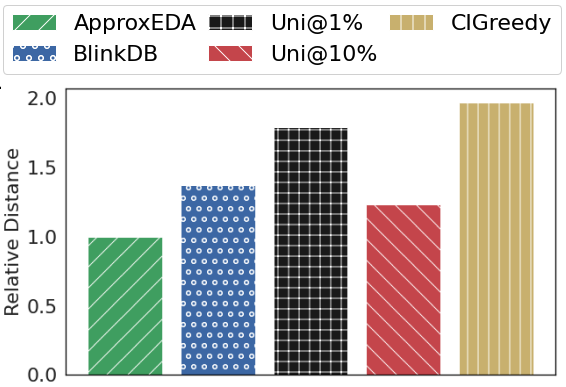
\includegraphics[width=1\linewidth]{LaTeX/figures/flights_eud.png}
\caption{Flights Dataset}
\end{subfigure}
\begin{subfigure}{\textwidth}
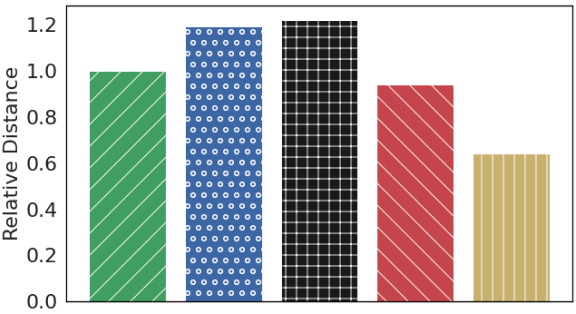
\includegraphics[width=1\linewidth]{LaTeX/figures/housing_eud.png}
\caption{Housing Dataset}
\end{subfigure}
\begin{subfigure}{\textwidth}
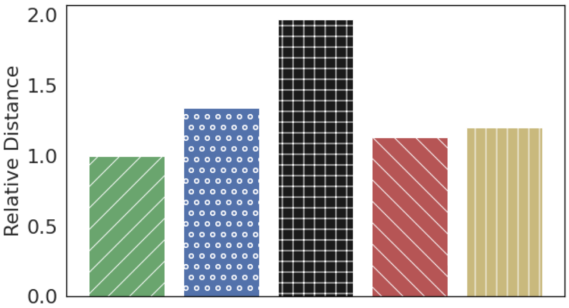
\includegraphics[width=1\linewidth]{LaTeX/figures/income_eud.png}
\caption{Income Dataset}
\end{subfigure}
\caption{Intent Divergence: Euclidean distance between original intent distribution and methods using samples. Normalized w.r.t. \name. Lower is better.}
\label{fig:rel_dist_1}
\end{minipage}%
\hfill
\begin{minipage}[t]{0.32\textwidth}
\begin{subfigure}{1\textwidth}
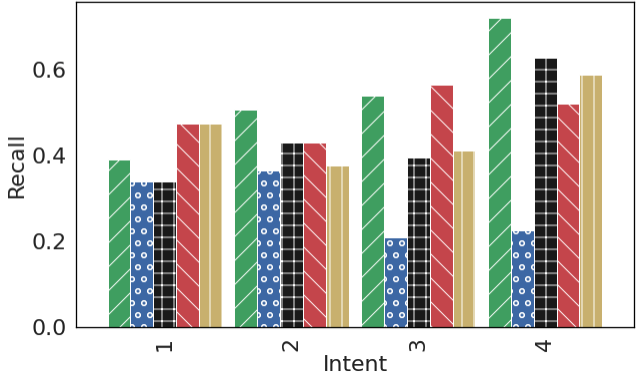
\includegraphics[width=1\linewidth]{LaTeX/figures/flights_intent1.png}
\caption{Flights Dataset}
\end{subfigure}
\begin{subfigure}{\textwidth}
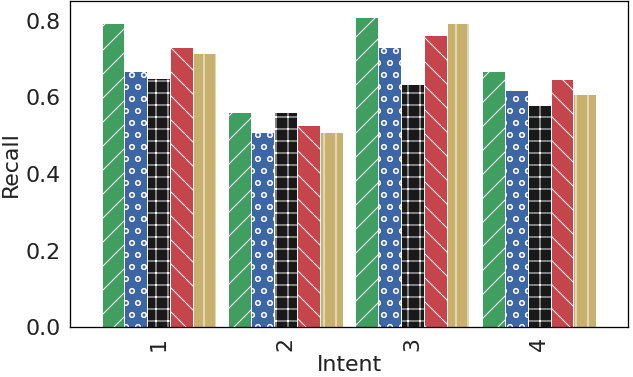
\includegraphics[width=1\linewidth]{LaTeX/figures/housing_intent.png}
\caption{Housing Dataset}
\end{subfigure}
\begin{subfigure}{\textwidth}
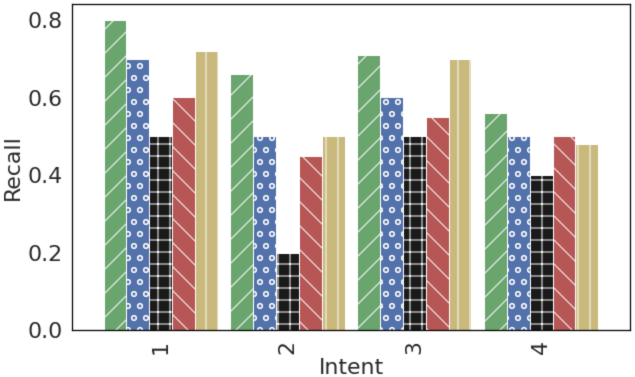
\includegraphics[width=1\linewidth]{LaTeX/figures/income_intent.png}
\caption{Income Dataset}
\end{subfigure}
\caption{Insight Preservation: Recall of the top 5 resulting rows at the end of analysis sequence compared to results from full data, across various intents. Higher is better.}
\label{fig:recall_5}
\end{minipage}%
\hfill
\begin{minipage}[t]{0.32\textwidth}
\centering
\begin{subfigure}{\textwidth}
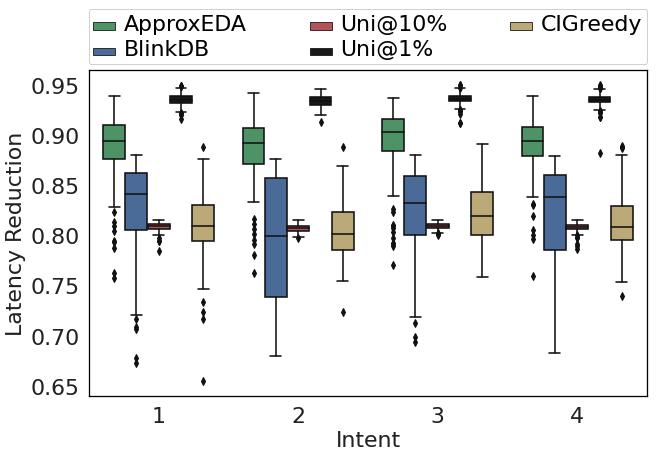
\includegraphics[width=1\linewidth]{LaTeX/figures/flight_lat.png}
\caption{Flights Dataset}
\end{subfigure}
\begin{subfigure}{\textwidth}
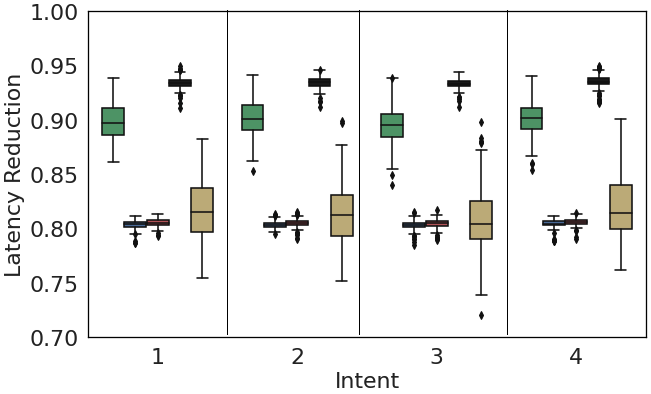
\includegraphics[width=1\linewidth]{LaTeX/figures/housing_lat_new.png}
\caption{Housing Dataset}
\end{subfigure}
\begin{subfigure}{\textwidth}
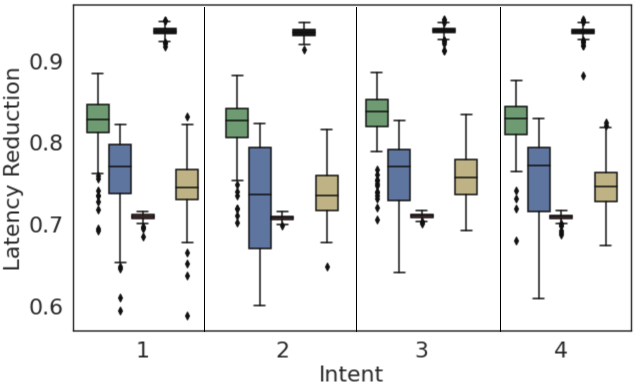
\includegraphics[width=1\linewidth]{LaTeX/figures/income_lat.png}
\caption{Income Dataset}
\end{subfigure}
\caption{The fraction of time saved by queries to run on the sampled dataset when using different models.
     Higher is better.}
     \label{fig:latency_reduction}
\end{minipage}%
%\hfill
\end{minipage}
\hfill
\begin{minipage}[t]{0.29\textwidth}
\centering
\begin{minipage}[t]{1.0\textwidth}
\centering
%\begin{table}
%\begin{center}
\scalebox{0.70}{
 \begin{tabular}[t]{|l|l|l|l|}
    \hline
    {Dataset} & {\# rows in full data} & {Unique sequences} \\
    \hline
    {Flights} & {5231403} & {10695}\\
    \hline
    {Housing} & {324196} & {6016} \\
    \hline
    {Income} & {426753} & {4032} \\
    \hline
    \end{tabular}
    }
 \captionof{table}{Dataset and EDA sequences}
 \label{tab:dataset}
%\end{center}
%\end{table}
\end{minipage}
\begin{minipage}[t]{1.0\textwidth}
\centering
 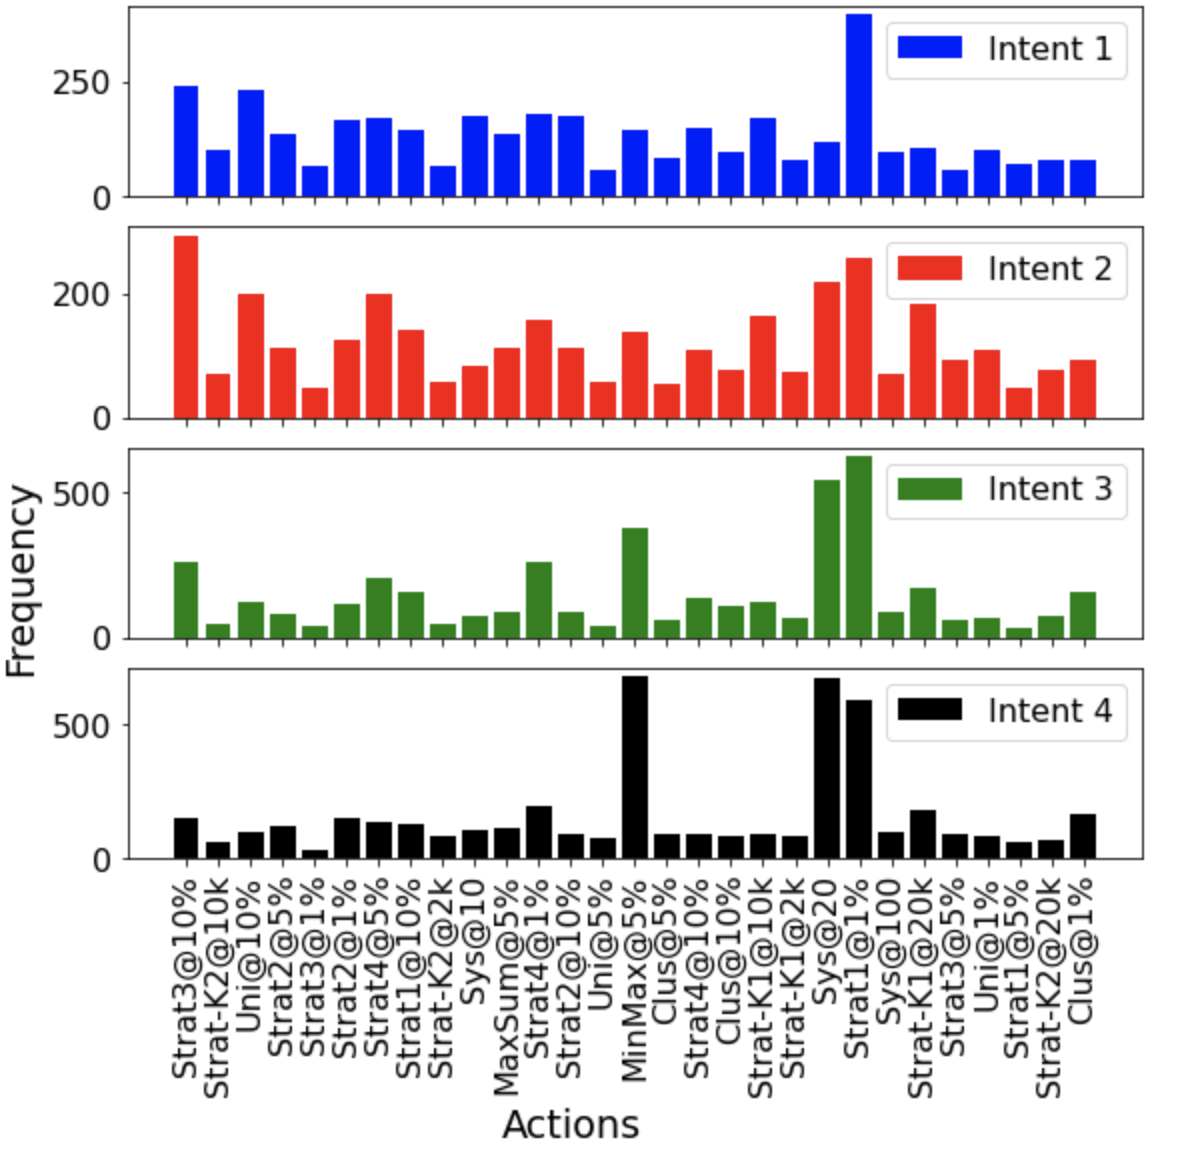
\includegraphics[width=\textwidth]{LaTeX/figures/intent_actions2.png}
      \caption{Frequency of different actions taken by \name for different intents.}
      \label{fig:action_usage}
 \end{minipage}
\end{minipage}
\vspace{-0.5em}
\end{figure*}


% \begin{figure*}[!t]
% \begin{minipage}[t]{0.4\textwidth}
% \begin{subfigure}{1\textwidth}
% \includegraphics[width=1.0\linewidth]{LaTeX/figures/Frame 50.png}
% \end{subfigure}
% \caption{Intent Divergence: Euclidean distance between original intent distribution and methods using samples. Normalized w.r.t. \name. Lower is better.}
% \label{fig:rel_dist_1}
% \end{minipage}%
% \hfill
% \begin{minipage}[t]{0.59\textwidth}
% \begin{subfigure}{1.0\textwidth}
% \includegraphics[width=1\linewidth]{LaTeX/figures/Frame 49 (2).png}
% \end{subfigure}
% % \begin{subfigure}{.3\textwidth}
% % 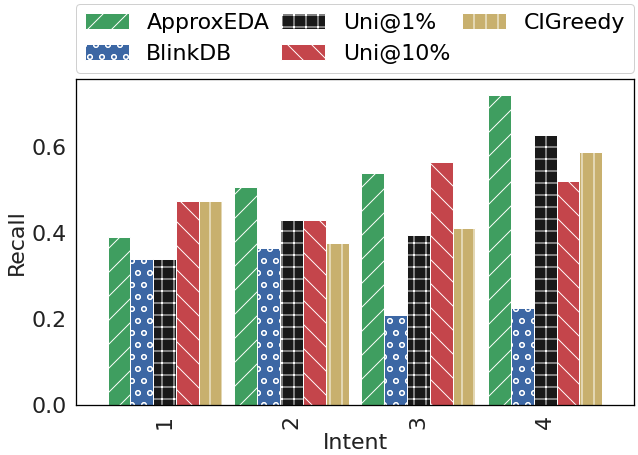
\includegraphics[width=1\linewidth]{LaTeX/figures/flights_5.png}
% % \caption{Flights Dataset}
% % \end{subfigure}
% % \begin{subfigure}{.3\textwidth}
% % 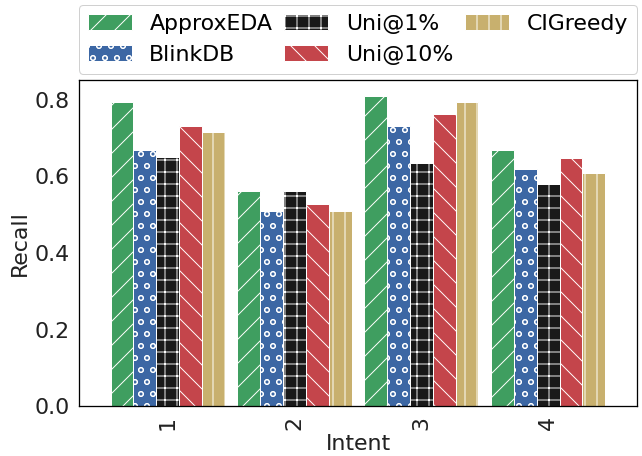
\includegraphics[width=1\linewidth]{LaTeX/figures/housing_5.png}
% % \caption{Housing Dataset}
% % \end{subfigure}
% % \begin{subfigure}{.3\textwidth}
% % 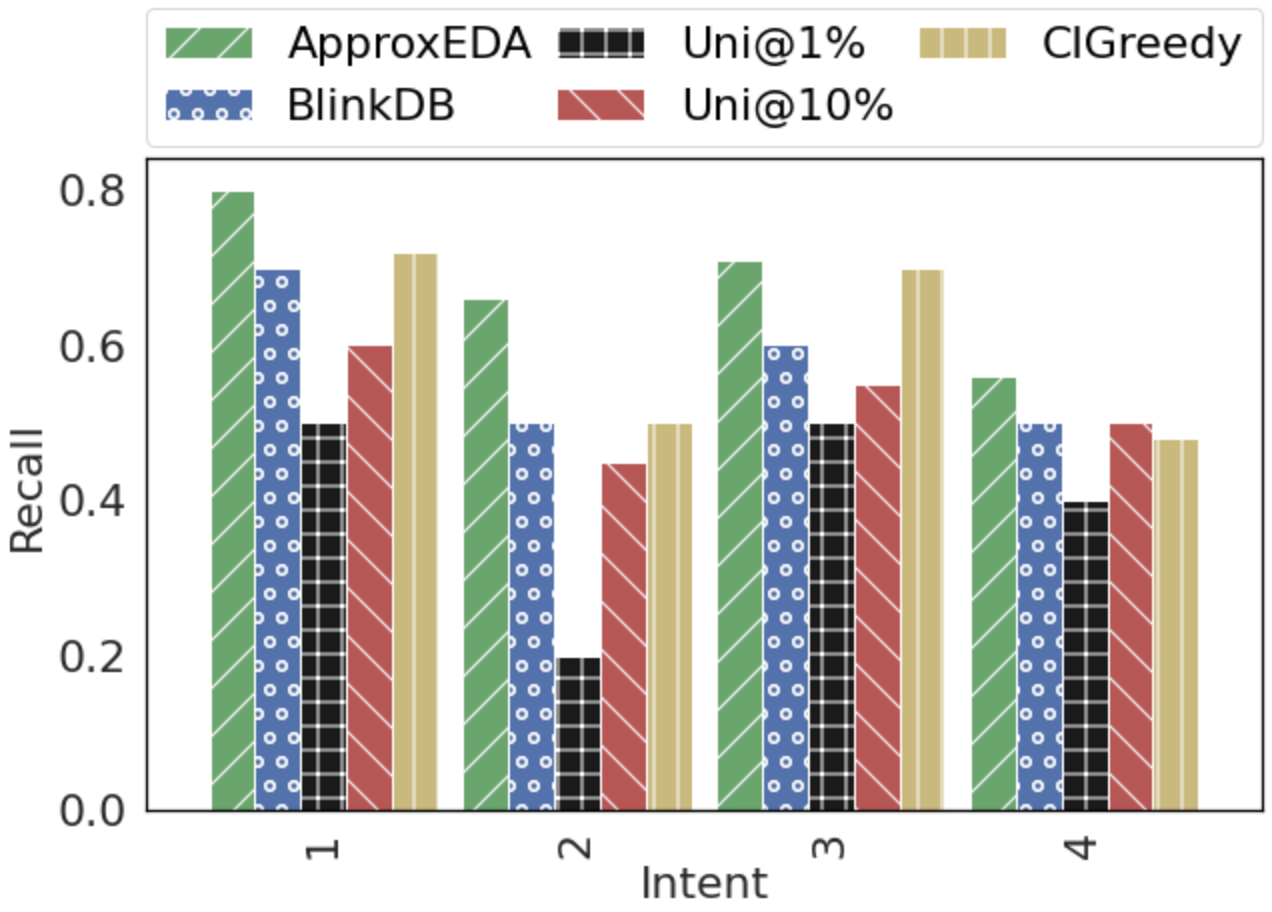
\includegraphics[width=1\linewidth]{LaTeX/figures/intent_preserve_income.png}
% % \caption{Income Dataset}
% % \end{subfigure}
%      \caption{Insight Preservation: Recall of the top 5 resulting rows at the end of analysis sequence compared to results from full data, across various intents.
%      Higher is better.}
%      \label{fig:recall_5}
% \end{minipage}
% \vspace{-1.0em}
% \end{figure*}


% \begin{table}[]
% \scalebox{1}{
% \begin{tabular}{|l|l|l|l|}
% \hline
%                  & \begin{tabular}[c]{@{}l@{}}EUD \\ (Zeta=0.25)\end{tabular} & 4.5  & 4.6   \\ \hline
% ApproxEDA        & 0.031                                                      & 0.12 & 0.728 \\ \hline
% BlinkDB          & 0.037                                                      & 0.11 & 0.73  \\ \hline
% Uniform          & 0.029                                                      & 0.10 & 0.45  \\ \hline
% CI\_Greedy       & 0.020                                                      & 0.11 & 0.40  \\ \hline
% CI\_Time\_Greedy & 0.022                                                      & 0.11 & 0.74  \\ \hline
% \end{tabular}
% }
% \captionof{table}{Results on the housing dataset}
% \label{tab:housing_results}
% \end{table}



\noindent\textbf{Baselines.}
%We compare with the following baselines:
\begin{itemize}
\item \noindent\textbf{\blink:}
%This is a state-of-the-art technique~\cite{agarwal2013blinkdb} for selecting a sample to get an approximate result for each individual query. 
\blink~\cite{agarwal2013blinkdb} attempts to minimize error for each query by selecting the stratified-sample that has the best overlap for QCS (explained before) of the
incoming query to be executed. 
When no overlap with stratified samples, we use 1\% uniform sample. 
%It does not have a notion of the intent or EDA sequences. 

\item \noindent\textbf{\greedy:}
We develop another intelligent baseline that first calculates a confidence interval (CI) for aggregate value requested by the incoming query on all the available samples (using a closed form formulation from~\cite{mozafari2015handbook}). 
Then chooses sample with the tightest CI at 95\% (i.e. indicating more confidence in the result).

\item \noindent{Uni@10\% and Uni@1\%:}
We compare our results with two other baselines where the agent always chooses a Uniform 10\% sample and Uniform 1\% sample respectively.
\end{itemize}

\noindent\textbf{Parameters.}
We use $K=4$ intents from BTM as it maximizes overall UCI score. Appendix~\ref{apps:intent_identification} and Figure~\ref{fig:intent_cluster} shows the clusters and UCI scores. We use values of $\beta$ and $\gamma$ as 1 to provide equal weightage to rewards after scaling them.
%\tong{this sentence may be moved to the experiment section?}

\subsection {Evaluation Methodology}
\label{sec:evaluation}
\vspace{-0.1em}
%
%While generation of these EDA sequences, we fix the first $k=3$ queries\footnote{We found usually first 3 or 4 queries and corresponding visualization set the experience analysts on a particular EDA flow particular initial queries From our domain experience}  
%\sm{Revisit this k=3 evaluation setup.}
%
%Note: only \name has the ability to do this selection in an intent-aware manner.
%
%\sm{Following may go in the ablation study.}
%For \name we present two sets of results: \textbf{seen} and \textbf{unseen}, when the held-out set is also used to learn the intents, and when it is not, respectively.



\begin{comment}
\begin{table}
\scalebox{0.8}{
 \begin{tabular}[ht!]{|l|l|l|c|}
    \hline
    {Sample Name} & {Short Name} & {Parameters} & {Effective SR}\\
    \hline
    {Uniform} & {Uni@$\tau$} & {$\tau$= [0.01, 0.05, 0.1]} & {[0.01, 0.05, 0.1]} \\
    \hline
    {Systematic} & {Sys@$k$} & {$k$= [100, 20, 10]} & {0.01, 0.05, 0.1]} \\
    \hline
    {Proportional stratified} & {Strat@$\tau$} & {$\tau$= [0.01, 0.05, 0.1]} & {[0.01, 0.05, 0.1]} \\
    \hline
    {At most $K$ stratified} & {Strat-K@$k$} & {$K$= [0.1]} & {[0.1]} \\
    \hline
    {Cluster} & {Clus@$k$} & {$k$= 10, $\tau$= [0.01, 0.05, 0.1]} & {[0.01, 0.05, 0.1]} \\
    \hline
    {Diversity} & {Div@$k$} & {$k$= 0.1*$|T|$} & {[0.1]} \\
    \hline
    \end{tabular}
    }
 \captionof{table}{Samples used as actions \sm{Make sure these parameter notations are explained in Sec-2.}}
 \label{tab:actions}
\end{table}
\end{comment}

\noindent\textbf{EDA Interactions using ATENA.}
%This is because data on which users perform such analyses are often proprietary. Moreover, the process being highly interactive and performed by proficient analysts, curating such a large volume of such data can be prohibitively costly. 
%
%We are the first to look at this problem of how to protect analysis intent divergence while using samples to speed up interactions. 
%As the problem of intent-divergence during EDA was not explored before, 
There are no public datasets available that combines both exploratory insight generation query sequences and the corresponding results on a given data that is also publicly available. 
Moreover, similar to many other interactive scenarios, such as conversational recommender systems \cite{christakopoulou2016towards}, dialog systems \cite{shi2019build,takanobu2020multi} and dialog-based interactive image retrieval \cite{guo2018dialog,yu2019visual}, a major challenge in the evaluation is that we need to have access to user reactions to any possible results returned by the system, which are exhaustive to collect in practice. Therefore, similar to \cite{christakopoulou2016towards,guo2018dialog,yu2019visual,shi2019build}, we adopt a setting where the user reactions are generated by simulators as surrogates for real users.
We overcome this by using an EDA simulator from prior work~\cite{atena2020sigmod}, called ATENA that is trained using real analysis sequences from expert analysts, which uses high-level statistical characteristics 
% (e.g. entropy, skew, \# unique categories etc.) 
of the data along with its schema structure 
% (e.g. numerical, categorical, primary-key column information) 
to generate realistic analysis sequence patterns similar human experts with various implicit intents~\cite{atena2020sigmod}.
%Similar to a real user, ATENA also formulates the next SQL query based on the previous set of queries that were run along with the corresponding results or displays (e.g. groups of rows from a \texttt{SELECT} or \texttt{GroupBy} query). Evaluations of ATENA show that the resulting query ordering and their coherence in the EDA sequences closely match with interactive analysis done by human experts on the same target dataset.  
%
%Specifically, 
%We use ATENA to both generate ideal exploratory sessions when no approximations through sampling is used, as well as to create interactive environment when samples are used and selected by our proposed RL-agent.
%
%This approach is similar to several prior works that used a simulator to evaluate a solution in an interactive setup~\cite{}. 
%\sm{Tong please specify few paper}.
%
%When training machine learning models of interactive systems, we usually use user simulators \citep{liu2018dialogue,shi2019build,guo2018dialog}.
%
%Similar to many other interactive scenarios, such as conversational recommender systems \cite{christakopoulou2016towards}, dialog systems \cite{shi2019build,takanobu2020multi} and dialog-based interactive image retrieval \cite{guo2018dialog,yu2019visual}, a major challenge in the evaluation is that we need to have access to user reactions to any possible results returned by the system, which are exhaustive to collect in practice. Therefore, similar to \cite{christakopoulou2016towards,guo2018dialog,yu2019visual,shi2019build}, we adopt a setting where the user reactions are generated by simulators as surrogates for real users.
For each of the datasets, we train this simulator following the methodology described in \cite{atena2020sigmod}.
Then we use this trained stochastic simulator to generate data exploration sessions which constitute sequence of queries and corresponding results or visualizations. 
For each dataset several such unique sequences can be generated by the simulator using multiple runs and is summarized in Table~\ref{tab:dataset}.
For each dataset, we set aside $1k$ sequences generated by the simulator using full data as held-out set for evaluations.
For \name and the baselines, we also generate $1k$ sequences by letting these methods interact with the simulator where for each query of the EDA, these methods select the optimal samples using their respective algorithms. 
%
Each of the sequences generated from any of the methods are fed into the BTM model to get the probability distribution of intents over the topics.

%\subsubsection{Metrics}

\subsection{Evaluation:Intent Divergence (RQ1)}
\label{sec:eval_intent}

We evaluate \name compared to the baselines in preserving the intent distributions (distribution of EDA interaction sequences over topic-models) of the original EDA sequences created without using any samples for approximations. 
%
In Figure ~\ref{fig:rel_dist_1} we present Euclidean Distance (ED) (normalized w.r.t. \name) between the intent distributions resulting from one of the baselines and from original unapproximated scenario. 
Lower ED is desirable as it indicates better matching of intent distribution. 
We can see that for Flights and Income, \name is best in preserving the distribution. 
For Housing it {Uni@10\%} (uniform sample at 10\%) and \greedy does better. 
This is because both {Uni@10\%} (uniform sample at 10\%) and \greedy ends up choosing large overall sample sizes, and hence less information loss and approximation error.  
However, in the following \S~\ref{sec:eval_latency} and associated latency improvement plot in Figure~\ref{fig:latency_reduction}, we see that such use of large samples makes these methods extremely poor for latency reduction and defeats the purpose of using samples to speed up interactivity. 
Supplement (\textbf{A.1}) provides the exact number of rows corresponding to each samples (actions) created by various sampling strategies.
%
%
%Since the EDA simulator we use is stochastic and \name intervenes with the simulator by providing samples to run the queries instead of the full original data --- it is not possible to exactly compare an EDA interaction sequence created while using \name with a particular \textit{ground truth sequence}.
%
%

\begin{comment}
The metric finally for n such sequences is the,
\begin{equation}
    Intent Accuracy = \frac{No. of correctly identified intents}{Total no. of sequences}
\end{equation}

\tong{Please follow notations from existing papers, instead of starting from scratch for the above equation.}

We evaluate how well the final insight of the EDA is preserved in addition to preserving the intent distribution. 
To do this, we define a metric Intent-Query-Coherence (IQC) that calculates the probability of a query, given its intent as follows:
\begin{equation}
    IQC(q_i | intent) = average(P(q_i | intent))
\end{equation}
across the test samples for a specified intent.

For this we use the last $k=2$ queries of the EDA sessions as representation of the \textit{final insight} that an analyst would use as key takeaways.

For last two queries generated by \name and baselines,
we calculate $X = \frac{IQC(Q_{L}) + IQC(Q_{L-1})}{2}$ the \textit{IQC} metric using $\argmax(P(S)$ as the given intent $I$ based on the resulting sequence $S$.
$L$ length of the EDA sequence.

Then we calculate a metric for final insight recall (FIR) for each method as:
Avg-over-each-generated-sequence($X$*Recall for results $Q_{l}$ and $Q_{l-1}$ over all sequences from $I$).

Recall is calculated over with k=3-5-10 rows in the result for each of the queries.
Precision is not important.

\end{comment}

\begin{figure*}[t!]
\begin{minipage}[t]{0.495\textwidth}
%\begin{table}[]
\scalebox{0.67}{
\begin{tabular}{|l|l|l|llll|}
\hline
\multirow{2}{*}{Model} & \multirow{2}{*}{\begin{tabular}[c]{@{}l@{}}Relative\\ ED\end{tabular}} & \multirow{2}{*}{\begin{tabular}[c]{@{}l@{}}Latency\\ Reduction\end{tabular}} & \multicolumn{4}{c|}{Overall Mean Recall}                                                                         \\ \cline{4-7} 
                       &                                                                              &                                                                              & \multicolumn{1}{l|}{Intent 1} & \multicolumn{1}{l|}{Intent 2} & \multicolumn{1}{l|}{Intent 3} & Intent 4 \\ \hline
\name                  & \textbf{1}                                                                            & 0.89                                                                         & \multicolumn{1}{l|}{0.32}     & \multicolumn{1}{l|}{\textbf{0.74}}     & \multicolumn{1}{l|}{0.29}     & 0.63     \\ \hline
\name - $R_{term}$     & 1.08                                                                         & \textbf{0.92}                                                                         & \multicolumn{1}{l|}{\textbf{0.39}}     & \multicolumn{1}{l|}{0.60}     & \multicolumn{1}{l|}{\textbf{0.32}}     & 0.38     \\ \hline
\name - $R_{intent}$   & 1.36                                                                         & 0.91                                                                         & \multicolumn{1}{l|}{0.31}     & \multicolumn{1}{l|}{0.57}     & \multicolumn{1}{l|}{0.30}     & 0.35     \\ \hline
\name - $R_{latency}$  & 1.12                                                                         & 0.83                                                                         & \multicolumn{1}{l|}{0.28}     & \multicolumn{1}{l|}{0.68}     & \multicolumn{1}{l|}{0.29}     & \textbf{0.68}     \\ \hline
\end{tabular}
}
\captionof{table}{Impact of different components of rewards.}
\label{tab:ablation_results}
%\end{table}
\end{minipage}%
\hfill
\begin{minipage}[t]{0.49\textwidth}
%\begin{table}[]
\scalebox{0.66}{
\begin{tabular}{|l|l|l|llll|}
\hline
\multirow{2}{*}{Action Space}                                             & \multirow{2}{*}{\begin{tabular}[c]{@{}l@{}}Relative\\ ED\end{tabular}} & \multirow{2}{*}{\begin{tabular}[c]{@{}l@{}}Latency\\ Reduction\end{tabular}} & \multicolumn{4}{c|}{Overall Mean Recall}                                                                         \\ \cline{4-7} 
                                                                          &                                                                              &                                                                              & \multicolumn{1}{l|}{Intent 1} & \multicolumn{1}{l|}{Intent 2} & \multicolumn{1}{l|}{Intent 3} & Intent 4 \\ \hline
Only Uniform                                                              & 1.34                                                                         & \textbf{0.90}                                                                         & \multicolumn{1}{l|}{\textbf{0.41}}     & \multicolumn{1}{l|}{0.60}     & \multicolumn{1}{l|}{0.28}     & 0.48     \\ \hline
Uniform + Stratified                                                      & \textbf{0.85}                                                                         & 0.84                                                                         & \multicolumn{1}{l|}{0.34}     & \multicolumn{1}{l|}{0.58}     & \multicolumn{1}{l|}{\textbf{0.30}}     & 0.65     \\ \hline
\begin{tabular}[c]{@{}l@{}}Uniform + Stratified \\ + Cluster\end{tabular} & 1.12                                                                         & \textbf{0.90}                                                                         & \multicolumn{1}{l|}{\textbf{0.41}}     & \multicolumn{1}{l|}{0.60}     & \multicolumn{1}{l|}{\textbf{0.30}}     & \textbf{0.66}     \\ \hline
All Samples                                                               & 1                                                                            & 0.89                                                                         & \multicolumn{1}{l|}{0.32}     & \multicolumn{1}{l|}{\textbf{0.74}}     & \multicolumn{1}{l|}{0.29}     & 0.63     \\ \hline
\end{tabular}
}
\captionof{table}{Ablation study: variations of action space.}
\label{tab:sample_results}
%\end{table}
\end{minipage}
\vspace{-0.8em}
\end{figure*}


\vspace{-0.2em}
\subsection{Evaluation: Insight Preservation (RQ2)}
\label{sec:eval_insight}
\vspace{-0.2em}

We evaluate how well the final insight of the EDA is preserved in addition to preserving the intent distribution.
Analysts usually derive insights at the end of each analysis sequence, using the outcome of the final few queries.
Since we do not have explicit labels about whether user actually received satisfactory insights at the end, we calculate a recall value based on results of row obtained from
different sampling based methods w.r.t. results obtained from use of full data.
To calculate this recall, we use top $k=5$ result rows obtained from last 2 queries from each of the analysis sequence -- a thumb rule we understood by talking to experts.

{\footnotesize
\begin{equation}
\label{recall_equation}
    Recall_{Intent=I} = \frac{|\bigcup_{i=1}^{n}M(Q_{i}) \cap \bigcup_{j=1}^{m}M(O_{j})|}{|\bigcup_{j=1}^{m}M(O_{j})|} , {Q_{i},O_{j}} \in I
\end{equation}
}

where $Q_i$ refers to the generated sequence, $O_j$ refers to the sequence generated on full data and $M(Q_i)$ is the union of the top $k$ results of the last two queries of the sequence $Q_i$.

Please note: the intent distribution (\S~\ref{sec:eval_intent}) along with this final insight preservation, as a combination ensures that users' do not diverge from their analysis workflow.  
This is because there can be hypothetical solutions that might directly match the results from last few queries, without replicating the intent of the analysis captured through the entire sequence of analysis. Even though, such a solution  would provide a high recall, but will fail to preserve the purpose of data exploration and associated understanding consumed by analysts~\cite{atena2020sigmod}. 
%
From Figure~\ref{fig:recall_5} we see that for 2 out of 4 intents for Flights data and all of the intents for Housing data and Income data, \name provides highest recall compared to the baselines. 
As explained in \S~\ref{sec:eval_intent}, the reason either {Uni@10\%} or \greedy sometimes provide higher recall because they end up choosing large sample sizes, which intern lead to much higher latency (Figure~\ref{fig:latency_reduction}). 
We also compute an \textit{overall recall} corresponding to all the results returned by the last 2 queries and illustrate in \ref{app:add_res}. 



\vspace{-0.2em}
\subsection{Evaluation:Latency Reduction (RQ3)}
\label{sec:eval_latency}
\vspace{-0.2em}

In Figure~\ref{fig:latency_reduction} we compare the latency improvement by \name compared to the other baselines. 
We compute the overall latency at a sequence level by summing up latency for each individual queries in that sequence. 
We calculate \% of reduction in sequence-level latency compared to the latency when each query execute against full data (y-axis: higher is better).
%
We show box-plots to show the distribution of values for each sequences, grouped by different intents. 
It can be observed that median sequence-level latency reduction for \name is almost 90\% (that is the analysis sequences take only $1/10^{th}$ of the original time.
%
Note: even though {Uni@1\%} provides most reduction as it always uses 1\% sample of the data irrespective of the context. 
Recall from Figure~\ref{fig:rel_dist_1} and ~\ref{fig:recall_5}, {Uni@1\%} is pretty bad in terms of preserving the intent distribution or the final insights. The combination of RQ1, RQ2 and RQ3 shows that \name's state can capture different context of sequential analysis and choose optimum trade-off space between statistical effectiveness of different samples vs. corresponding latencies.

 
% \tong{need some notations. Please follow notations from existing papers, instead of starting from scratch for the equation.}



\vspace{-0.2em}
\subsection{Qualitative Evaluation}
\vspace{-0.2em}
%
Due to space, in Appendix~\textbf{\ref{apps:qualitative_eval}} Figure~\ref{fig:real} we show a real EDA session with \name to illustrate in-spite of it selecting frugal samples at various points (e.g. Clus@1\%, Uni@5\% etc.), \name can mostly preserve the query structure, analysis sequence and final outcome/insight. 
In Figure~\ref{fig:action_usage} we show the variation of \name's choice of different actions (selection of samples) for 4 different intents identified for the Flights data across all the held out sequences.
We found that certain samples (e.g. MaxMin@5\%, Sys@20\%, Strat1@1\%) were predominantly chosen for certain intents (e.g. \#4). Intuition is that such samples can preserve representations of smaller groups better, which is necessary for that intent preservation.

\subsection{Ablation Study}
%
We conduct an ablation study to illustrate the effect of each component on the final metrics in Table~\ref{tab:ablation_results}.
The show Relative-ED, Latency-Reduction and Mean-Overall-Recall as the metric. We progressively remove one reward at a time and see the effect it has on the metrics. Comparing \name and \name - $R_{term}$ , we observe that the latency reduction increases. This is because $R_{latency}$ now has a greater impact on the total reward. However, this is accompanied by a sharp decrease in the Mean Recall value for Intent 2 and Intent 4 as this metric is highly dependant on $R_{term}$. The increase in mean recall for Intent 1 and Intent 3 is nominal.
%
Removing the $R_{intent}$, we notice that the model now performs worse on every metric except latency. This is because both Relative ED and Mean Recall are highly intent dependant and the lack of intent reward makes it difficult for model to learn a good enough distribution. The improvement in latency can be credited to the higher weight of the latency reward as seen in earlier the earlier case. 
%
We then verify the effect of removing $R_{latency}$. As expected, we observe that the latency reduction has largely dropped and thus the agent trained without $R_{latency}$ is free to choose larger samples in order to maximise the reward. We notice that, the model now  performs similar to \name and is better in terms of Metric Recall on Intent 4.
Table~\ref{tab:sample_results} shows sensitivity of \name w.r.t. to availability of different groups of sampling algorithms in its action space.

\begin{table}[th]
\tiny

\label{table:ablation_delta}
\begin{tabular}{|l|l|l|llll|}
\hline
\multicolumn{1}{|c|}{\multirow{2}{*}{\begin{tabular}[c]{@{}c@{}}Model \\ Parameter\end{tabular}}} & \multicolumn{1}{c|}{\multirow{2}{*}{Relative ED}} & \multicolumn{1}{c|}{\multirow{2}{*}{\begin{tabular}[c]{@{}c@{}}Latency \\ Reduction\end{tabular}}} & \multicolumn{4}{c|}{\begin{tabular}[c]{@{}c@{}}Mean Overall\\  Recall\end{tabular}}                                           \\ \cline{4-7} 
\multicolumn{1}{|c|}{}                                                                            & \multicolumn{1}{c|}{}                             & \multicolumn{1}{c|}{}                                                                              & \multicolumn{1}{c|}{Intent 1} & \multicolumn{1}{c|}{Intent 2} & \multicolumn{1}{c|}{Intent 3} & \multicolumn{1}{c|}{Intent 4} \\ \hline
$\delta =1$                                                                                         & 1                                                 & 0.89                                                                                               & \multicolumn{1}{l|}{0.32}     & \multicolumn{1}{l|}{0.74}     & \multicolumn{1}{l|}{0.29}     & 0.68                          \\ \hline
$\delta = 0$                                                                                        & 1.2                                               & 0.90                                                                                               & \multicolumn{1}{l|}{0.31}     & \multicolumn{1}{l|}{0.61}     & \multicolumn{1}{l|}{0.3}      & 0.42                          \\ \hline
\end{tabular}
\caption{Ablation study: Variation of $\delta$ in $R_{intent} = R_{dis} + \delta*R_{topic}$ (Ref. \S~\ref{sec:reward}).}
\label{tbl:ablation_delta}
\end{table}

We also do an ablation study on  $\delta$ and show the same in Table~\ref{tbl:ablation_delta}.
We observe that both components of our reward are important. Setting $\delta=0$ increases our relative distance between distributions. Although it reduces the latency, the gain is small. We also see that for various intents, our recall decreases significantly for Intent 2 and Intent 4. This is because setting $\delta=0$ removes the component that matches intent of the original sequence with the generated.

%\subsection{Discussion}
%\sm{Details/discussions on why the RL-based approach does better than baselines such as BlinkDB and others?
%
%It’s always an accuracy vs latency trade off, and the paper should motivate and demonstrate that the RL-based approach leads to more accuracy in less time compared to baselines.
%
%“The authors do not sufficiently discuss the downsides of an intent-aware sampling approach. For example, the proposed strategy introduces a bias towards, unlike its main competitors that sample uniformly at random. Consequently, it remains unclear whether the proposed method can estimate a truly exploratory user intent, as it will be more random (ln. 118). The introduced bias appears to be more problematic than the accumulated approximation error.”
%However, the query can be highly diverse. It means training a reliable policy in the proposed deep RL is hard by itself. Since the motivation of sampling is processing efficiency and in turn this paper aims to address the issues due to sampling, the impact of the RL must be evaluated



\begin{comment}

\subsubsection{Precision/Recall}
This captures the precision and recall numbers for the top $m$ groups in the result of last $k$ queries of the sequence. The analyst may reach the same state by different paths and the last $k$ queries are the most important for the exploration and we want the results to be as close as possible. \tong{need some notations. Please follow notations from existing papers, instead of starting from scratch for the  equation.}

\subsection{Results and Analysis}
\colorbox{yellow}{Experiment section 4:} 
\begin{itemize}
    \item Find a greedy baseline
    \item Find the closest paper and modify it to suit to our needs
    \item Find an evaluation metric and compare the following things on this metric:
        \begin{itemize}
            \item Greedy vs Published vs Our Method (best performing model) for 3 datasets
            \item Intent identification accuracy numbers for original vs fixed vs agent when first k queries out of n are fixed and rest are generated by simulator from these strategies.
            \item For a fixed sample, percentage savings over the original compared to some fixed strategies. 
            \item Ablation study experiment results
            \item Experiment with various RL algorithms like PPO/AUC and show the convergence properties.
            \item Look into what TBleu does and see if it can be useful
            \item Somehow fix last 2-3 queries and then compare
        \end{itemize}



\end{itemize}
\end{comment}
%\vspace{-0.5em}
\section{Related Works}
%\vspace{-0.3em}
\noindent\textbf{Intent Analysis and Understanding: }
%
Several papers dealt with the concept of
intents or goals for recommendations in process mining, web mining, education~\cite{jiang2019time, jiang2019goal} and analyze patterns in user behavior from application log/clicks data~\cite{aggarwal2020goal, dev2017identifying} or characterised SQL query logs to understand analysis behaviors~\cite{jain2016sqlshare}. 
%They do not consider the results for each of the those queries that might have influenced the patterns.
Distinct from all these, we identify goal as a combination of queries and the corresponding results in a sequential decision making workflow.

\noindent\textbf{Data Exploration:}
%
\cite{brachmann2019data} simplified
the manual creation EDA notebooks, cite{chirigati2016data} focused on related dataset recommendation. \cite{zhao2017controlling} attempts to flag false discoveries in EDA automation but does not consider approximations or intent of analysts.
%
Recent work also focused on automatically generating  data insights~\cite{ma2021metainsight, ding2019quickinsights} or creating or augmenting EDA workflows~\cite{atena2020sigmod, kery2018story, rule2018exploration}. 
%As an orthogonal direction, we focus on faster exploration with intent-aware use of approximations.
Several papers used samples and approximate query processing to speed up data explorations and analytics~\cite{sheoran2022aaai, sheoran2022electra, babcock2003dynamic, chaudhuri2017approximate, ma2021learned, bater2020saqe} but we are the first to look at the sequence and context of such exploration for visual analytics. 

%\noindent\textbf{Sampling and Approximations:} 
%
%\cite{park2016visualization} proposed a sampling strategy that guarantees high quality visualizations with a small subset of the entire dataset. But they do not consider interactive and sequential decision making workflow. 
%Several works~\cite{moritz2017trust, zhao2018random, agarwal2013blinkdb, park2018verdictdb} developed techniques for sampling to reduce error for ad-hoc queries, and make them compute efficient~\cite{ding2016sample, peng2018aqp}. We used several of these sampling techniques in our action space.

\noindent\textbf{Interactive Applications by Reinforcement Learning}
%The recent advances of reinforcement learning and deep learning enables many novel interactive applications.
\citet{liu2018dialogue,takanobu2020multi} propose interactive dialog systems based on reinforcement learning.
\citet{guo2018dialog} propose a dialog-based interactive image retrieval system involving natural language feedback on visual attributes of the items.
%Instead of searching for simple images,
\citet{tan2019drill} propose reinforcement learning with a drill-down method to interactively retrieve complex scene images.
Reinforcement learning from reformulations is proposed for question answering, by modeling the answering process as multiple agents walking in parallel on the knowledge graph \cite{kaiser2021reinforcement}.  \citet{hua2020few} propose
a meta reinforcement learning method in complex question answering, which quickly adapts to unseen questions. 
Reinforcement learning has also been applied to elicit user preferences in conversational recommender systems \cite{christakopoulou2016towards, zhang2020conversational,lei2020interactive}. Similar to these interactive scenarios \cite{guo2018dialog,yu2019visual,takanobu2020multi}, a major challenge in the evaluation is that we need to have access to user reactions to any possible results returned by the system, which are exhaustive to collect. Therefore, similarly, we adopt a setting where the user reactions are generated by simulators as surrogates for real users as detailed in Section \ref{sec:evaluation}.

%\noindent\textbf{Temporal Question Answering}
%\sm{Missing discussion of the related work in “temporal question answering”}
%\tong{not sure whether we need a separate section}
%\tong{Please summarize some relevant papers.}
%\sm{Tong: Please write about use of RL and simulators in a wide range of domains like image captioning, NLP etc.}


\section{Conclusions}

We proposed a deep RL based technique to optimize exploratory data analytics using down-sampled data.  
Our intelligent and contextual sample selection can prevent misleading explorations and insights while still ensuring lower latency of interactions. Evaluations show that our method is superior to baselines when used on three real-world dataset.   


\newpage
%\newpage
%%% BIBLIOGRAPHY

\vspace{-0.5em}
%{\footnotesize
%\bibliographystyle{ACM-Reference-Format}
\bibliography{biblio}
%}

\newpage
\appendix
\clearpage
\section{Supplemental Information}

\begin{algorithm}[th]
        \begin{algorithmic}[1]
        \label{alg:alg1}
        \caption{\name{}'s Training Algorithm}
        % \textbf{Input} Dataset $D$
        \STATE Train the ATENA~\S{5.2} on given dataset $D$
        \STATE Generate sequences $O$ using ATENA
        \STATE Train a $BTM$ model $\phi$ with $K$ topics on $O$
        \STATE Create sample set $A=\{a_1,a_2,...,a_i\}_{i=1}^n$
        \STATE Initialise A2C model
        \FOR{$i = 1,...,episodes$}
            \STATE Initialize the state space $s_t$ as in (\ref{eq:state_space}) with zeroes
            \FOR{$t = 1,...,l$}                    
                    \STATE Generate a query $q_t$ from the simulator
                    \STATE Take action $a_t$ for the given $s_t$
                    \STATE Update $s_t$ with latest query $q_t$, display vectors $v_t$, latency $C_t$ and current intent as $\phi(Q_t)$
            \ENDFOR
            \STATE Calculate Individual rewards using~\S{4.3}.
            \STATE Calculate the total reward $R_t$
            \STATE Calculate $J_R(\pi) = \mathbb{E}_{a_t \sim \pi_\theta}[R_t]$
            \STATE Compute loss functions $\mathbb{L}(\theta)$ for policy network
            \STATE Compute $\mathbb{L}(\omega)$ for value network
            \STATE Update A2C model
        \ENDFOR
        \end{algorithmic}
    \end{algorithm}

\subsection{Formal Problem Formulation}
\label{sec:problem}
%
%\sm{Please review. Does this problem formulation make sense or does it becomes confusing or conflicting}


%
%\tong{Is $D$ the variable $A$ in Section 4.1?}
%\sm{Yes}
Let $D_0$ be the full data target for EDA.
Let $D'$ = $\{D_i\}_{i=1}^n$ be $n$ subsamples created from $D$ and $|D_i| < |D_0|$ for $i \in [1, n]$ where $|.|$ denotes size (\# of rows). 
Let an $l$ length EDA session $e=\langle \{q_j(D_i), v_j(D_i)\}_{j=1}^l | i \in [1,n]\rangle$ be comprised of an alternating sequence of queries $q_j(.)$ and corresponding results/visual output $v_j(.)$ performed on data $D_i$. 
Note $D$ is the variable $A$ in Section 4.1 and line 4 of Algorithm 1.
%

Let $I$ be the set of implicit intents embedded in the distribution of all $e$, the EDA sessions.
%\sg{What is e here?}\sm{e is an EDA sequence/session}
%
Let $I^{D_0}$ be original distribution of the intents $P(I|D_0)$, i.e. when all EDA was done using full data $D_0$.
Let $I^{D'}$ be the distribution $P(I|D')$, i.e., EDA is approximated using only subsamples.
Our goal is to find optimal subsample $D_i, i \in [1,n]$ for each step of the EDA $\{q_j(.), v_j(.)\}$ such that $Div(I^{D_0}||I^{D'})$ is minimized with $I$ as the support.
%

We define $Div(I^{D_0}||I^{D'})$ as the \textbf{intent-divergence} between the EDA performed using full data and approximate EDA using only subsampled data. 

\subsection{Discussion: Intent-divergence vs. intent-shift}
\label{app:discussion_intent_shift}

Please note, in this paper we address the problem of \textit{intent-divergence} where the users' have a set of consistent implicit objectives/intents during the EDA. 
While \name{} deliberately introduces a bias towards a set of intents inferred from historical analysis sequences, this is justified as real expert users often follow some standard exploration strategies and look for similar types of insights even on new datasets as observed by multiple prior works~\cite{atena2020sigmod, jain2016sqlshare, milo2018next} and do not perform random explorations.
However, if such implicit objectives suddenly change causing an \textit{intent-shift}, then \name{}'s current design would not be able to detect that. 
In this paper, it is assumed that there is limited \textit{intent-shift} (\emph{i.e.}, change of user's core intent characteristics). 
%While in this paper we are the first to address how to prevent intent-divergence (approximation errors misleads users to a different intent), 
This assumption is widely adopted in other interactive applications \cite{liu2018dialogue,guo2018dialog,tan2019drill}, although it is interesting to address the intent-shift \cite{xie2021tiage,arnold2019sector}. As the first work on approximate exploratory data analysis in the interactive setting, we leave addressing \textit{intent-shift} as future work.


\begin{figure*}[!t]
\centering
\begin{minipage}[t]{0.57\textwidth}
\vspace{0pt}
\begin{subfigure}{.5\textwidth}
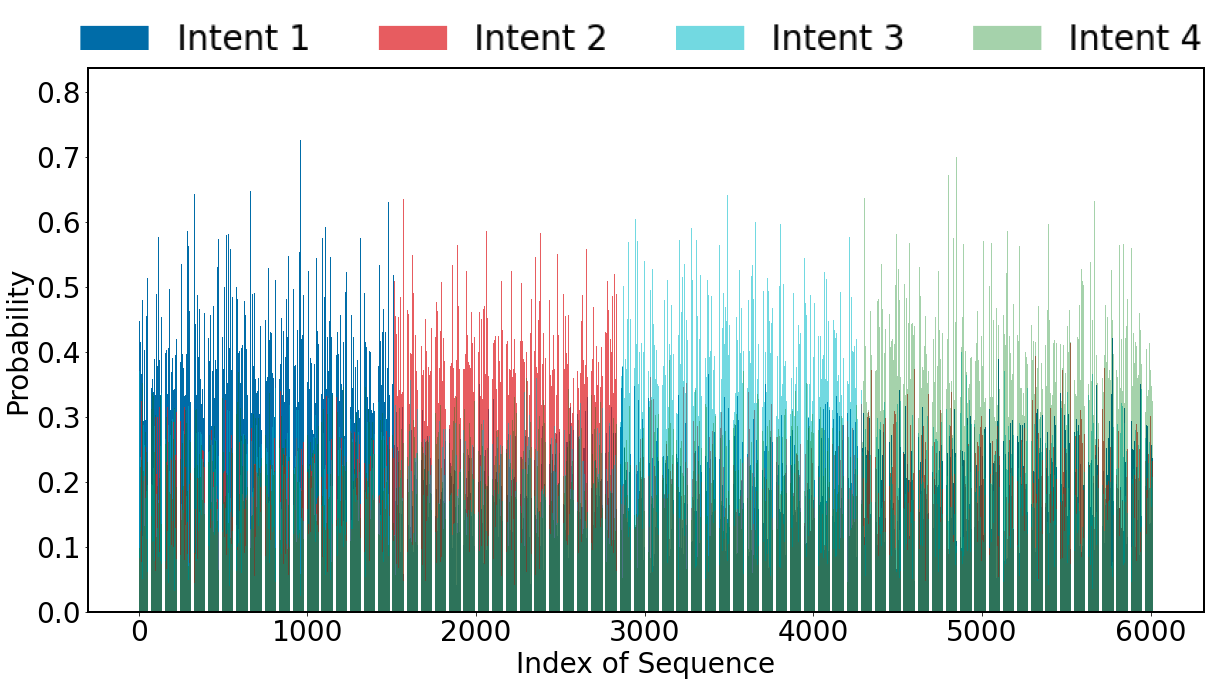
\includegraphics[width=1.0\linewidth]{LaTeX/figures/intentcl1.png}
\caption{EDA on Flights Dataset}
\end{subfigure}
\begin{subfigure}{.5\textwidth}
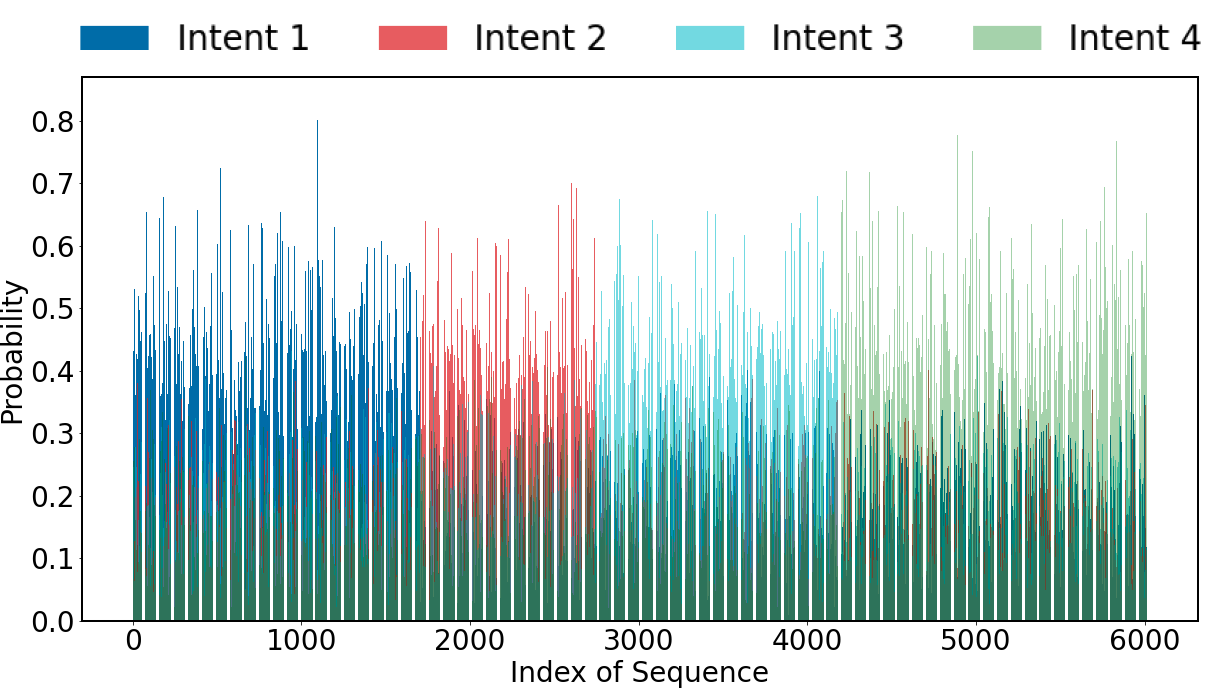
\includegraphics[width=1.0\linewidth]{LaTeX/figures/intentcl2.png}
\caption{EDA on Housing Dataset}
\end{subfigure}
     \caption{The probability distribution of query sequences for each of the identified $k=4$ intents. The sequences are grouped together intent-wise. This graph illustrates the distinguishable definitions of intents through their probability distributions. Since trend on Income dataset is similar, we omit the details.}
     \label{fig:intent_cluster}
\end{minipage}
%\hfill
\hspace{0.05\textwidth}
\begin{minipage}[t]{0.37\textwidth}
\vspace{0pt}
\begin{subfigure}{1.0\textwidth}
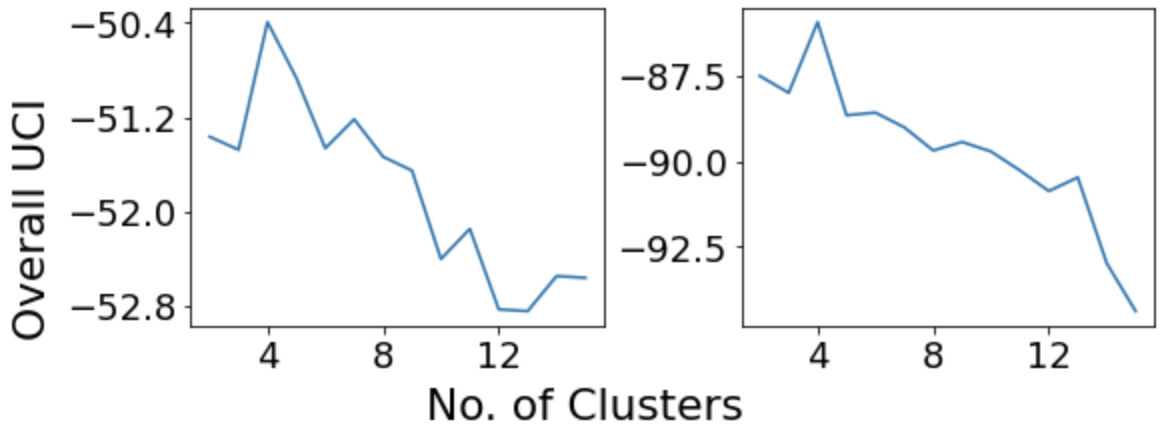
\includegraphics[width=1.0\linewidth]{LaTeX/figures/uci_plot_new.png}
%\caption{UCI measure for different number of cluster}
\end{subfigure}
\caption{UCI measure for different number of clusters (Left: Flights, Right: Housing data). Overall UCI is the highest when $K=4$ for both. Since trend on Income dataset is similar, we omit the details.}
     \label{fig:intent_clusters}
\end{minipage}
%\begin{minipage}[t]{0.2\textwidth}
%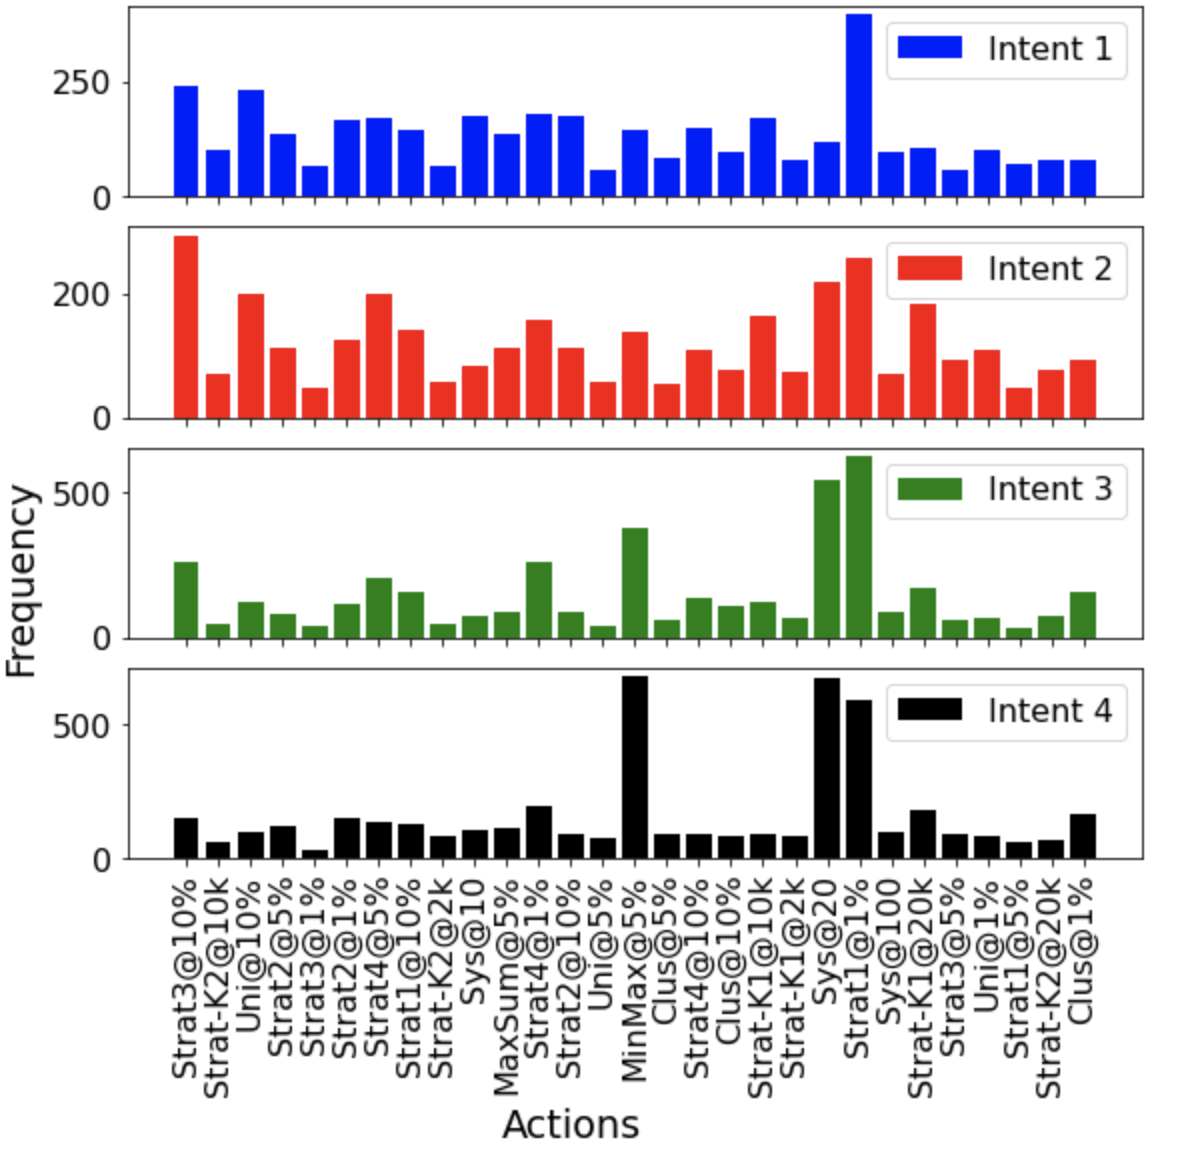
\includegraphics[width=\linewidth]{LaTeX/figures/intent_actions2.png}
%     \caption{Frequency of different actions taken by \name{} for different intents.}
%     \label{fig:action_usage}
%\end{minipage}
\vspace{-0.5em}
\end{figure*}

\subsection{Discussions: Design and Deployment}
\label{app:discussion}

\noindent\textbf{RL vs. Greedy Solutions.}

Simple greedy solutions would not work because because of the following reasons:
(1) It is impossible to calculate an approximation error when a query is run against each of the samples, unless we also run it against the original data at run-time (which defeats the purpose of using samples), 
(2) Even if we calculate an estimate of the approximation error, choosing the sampling strategy that minimizes error for each query may not be optimal because a less-accurate strategy might be of significantly lesser size, but still contain enough information that would preserve the high-level signal in the results (e.g. a bar being substantially higher than the rest) and would not lead to a wrong decisions by the analyst while choosing subsequent queries.

\noindent\textbf{Deployment Aspects.}

Significant history of EDA analysis sequence gets generated for data analysis usecases related to e-commerce, web/mobile analytics or digital marketing setting, where several analysts repeatedly explore the data to constantly understand different aspects of customer behavior. 
%At certain intervals, more recent data is ingested in batch and appended with the existing data causing the data-size to become significantly larger over time. 
%
In production scenario, different samples  are periodically regenerated in an offline manner as new batch of data of significant size is ingested. 
However, according to our understanding from experts, the EDA analysis patterns and intents for a particular dataset remains same over time (also refer to \S~\ref{app:discussion_intent_shift}).
Since, the overall characteristics of intents of the analysts do not change, \name{}'s learning about the effectiveness of different samples under different contexts does not get significantly affected if the overall statistical characteristics of the freshly ingested data is consistent with the old one.
However, if the statistical characteristics change, then \name{} is retrained with new samples in the background and after convergence the old model is replaced. 



\subsection{More Ablation Study Results}

\begin{table}[th]
\tiny

\label{table:ablation_delta}
\begin{tabular}{|l|l|l|llll|}
\hline
\multicolumn{1}{|c|}{\multirow{2}{*}{\begin{tabular}[c]{@{}c@{}}Model \\ Parameter\end{tabular}}} & \multicolumn{1}{c|}{\multirow{2}{*}{Relative ED}} & \multicolumn{1}{c|}{\multirow{2}{*}{\begin{tabular}[c]{@{}c@{}}Latency \\ Reduction\end{tabular}}} & \multicolumn{4}{c|}{\begin{tabular}[c]{@{}c@{}}Mean Overall\\  Recall\end{tabular}}                                           \\ \cline{4-7} 
\multicolumn{1}{|c|}{}                                                                            & \multicolumn{1}{c|}{}                             & \multicolumn{1}{c|}{}                                                                              & \multicolumn{1}{c|}{Intent 1} & \multicolumn{1}{c|}{Intent 2} & \multicolumn{1}{c|}{Intent 3} & \multicolumn{1}{c|}{Intent 4} \\ \hline
$\delta =1$                                                                                         & 1                                                 & 0.89                                                                                               & \multicolumn{1}{l|}{0.32}     & \multicolumn{1}{l|}{0.74}     & \multicolumn{1}{l|}{0.29}     & 0.68                          \\ \hline
$\delta = 0$                                                                                        & 1.2                                               & 0.90                                                                                               & \multicolumn{1}{l|}{0.31}     & \multicolumn{1}{l|}{0.61}     & \multicolumn{1}{l|}{0.3}      & 0.42                          \\ \hline
\end{tabular}
\caption{Ablation study: Variation of $\delta$ in $R_{intent} = R_{dis} + \delta*R_{topic}$ (Ref. \S~\ref{sec:reward}).}
\label{tbl:ablation_delta}
\end{table}

Recall in \S~\ref{sec:reward}, we use full intent reward as: $R_{intent} = R_{dis} + \delta*R_{topic}$.
We do an ablation study on this $\delta$ and show in Table~\ref{tbl:ablation_delta}.
We observe that both components of our reward are important. Setting $\delta=0$ increases our relative distance between distributions. Although it reduces the latency, the gain is small. We also see that for various intents, our recall decreases significantly for Intent 2 and Intent 4. This is because setting $\delta=0$ removes the component that matches intent of the original sequence with the generated.

\begin{table}[]
\scalebox{0.8}{
\begin{tabular}{|l|l|}
\hline
No. of Intents & \begin{tabular}[c]{@{}l@{}}Relative  ED\end{tabular} \\ \hline
4              & 1                                                     \\ \hline
6              & 2.98                                                  \\ \hline
8              & 5.84                                                  \\ \hline
10             & 7.41                                                  \\ \hline
\end{tabular}
}
\caption{Ablation study: Variation of K or \# of intents (Ref ~\S{\ref{sec:intent_identification}})}
\label{tbl:ablation_K_intent}
\end{table}

In Table~\ref{tbl:ablation_K_intent} we show ablation study for Flights dataset on number of intents used ($K$) (Ref. ~\S{\ref{sec:intent_identification}}) and how Euclidean Distance (ED) from ideal changes (increase in ED is worse) relative to the distance for number of intents $K=4.$

% Please add the following required packages to your document preamble:
% \usepackage{multirow}


\subsection{Intent Identification Results} 
\label{apps:intent_identification}


Figure~\ref{fig:intent_cluster} shows the probability distribution of intents for each of the query sequence and the 4 clusters identified can be clearly observed for Flights and Housing datasets. 
Since trend on Income dataset is similar, we omit the details.
To choose the best value for the number of intents, $K$, we compute the overall UCI score for all $K \in [2,15]$ and choose the best K. As can be seen maximum UCI score is observable at K=4.
%\tong{this sentence and figures may be moved to the appendix?}

\subsection{Model and Implementation Details}
\label{apps:model_implementation}
% \tong{I merged two appendix sections into one section. Please make sure the original referred appendix section ID is still valid in the paper content (i.e., first 9 pages).}
Our approach is based on A2C, an actor critic model for the training of our RL Agent. An actor critic model consists of two parts, an actor (policy network) which takes the state of the agent and outputs the best possible action, whereas the critic (value network) evaluates the action by computing the value function. %These two networks incrementally get better at their roles and the resultant architecture is better than the two methods separately.

%To train our A2C model, we use two separate networks. The policy network is a fully connected neural network and its task is to produce the best action given the agent state. The value network is also a fully connected neural network, and it receives the input as the state of the agent and the action chosen by the policy and outputs the Advantage value. This advantage value is the estimate of how good the chosen action can be in future. The training of both the networks happens separately and it uses gradient ascent to update the weights. The update of weights happen at each step (TD Learning).

To train our model, we generate 10k sequences using the simulator~\cite{atena2020sigmod} and we get 5995 unique sequences for the flights dataset and 6016 sequences for the housing dataset. We use $K=4$ for our experiments. To train the RL agent, for both policy network and value network, we use neural networks consisting of 2 fully-connected layers, with a dimension of 64 each. The activation function used is $\tanh$. The policy model used is MlpPolicy and we set the number of environments to 64. For the A2C model, we set the value function coefficient, $vf_{coef} = 0.25$ and the entropy coefficient, $ent_{coef} = 0.01$. The learning rate used for the model is 0.0007. More details about the algorithm are explained in \S{\ref{app:training}}
 
For the reward calculation, we scale all the rewards between $[-0.5, 0.5]$. For training \name{}, we used $\delta=1, \zeta=1$. To give equal weight to all the reward components, we set the value of $\beta=0.5, \gamma=0.5$. \ref{tab:model-details} shows some details for the trained model.

Tables \ref{tab:flights_samples}, \ref{tab:housing_samples} and \ref{tab:income_samples} show the actual number of rows sampled from each dataset and presents the Effective Sampling Rate (ESR). We create 29 samples for the \textit{Flights dataset} as shown and create 15 samples for each of \textit{Housing dataset} and \textit{Income dataset}.
In Figure~\ref{fig:my_conv} we show the training convergence curves. For evaluation, we choose the model with the best possible reward. The no. of steps for selection of the model is given in Table 7.

\begin{table}[H]
\vspace{0pt}
\scalebox{1}{
\begin{tabular}{|l|l|l|l|}
\hline
Dataset & \begin{tabular}[c]{@{}l@{}}No. of \\ steps\end{tabular} & Time(hr) & Model Size(KiB) \\ \hline
Housing & 36k                                                       & 20.3     & 284       \\ \hline
Flights & 36k                                                       & 15.8     & 363       \\ \hline
Income & 33k                                                       & 16.7     & 312       \\ \hline
\end{tabular}
}
\caption{Training times and model sizes}
\label{tab:model-details}
\end{table}
 
\subsection{Training Algorithm}
\label{app:training}
% \tong{I slightly changed the following algorithm. Please check whether the updated version looks good.}
Algorithm 1 explains the steps we use for training our RL Agent. It takes in the dataset $D$, processes it by creating samples as shown in line 4 and training ATENA simulator on the same as shown in line 1. Then on the generated sequences, a BTM model is trained in line 3. Once this is done, we then start the training of our agent as demonstrated in lines 5-18 of Algorithm 1. We follow episodic training where we calculate rewards at the end of each episode as shown in line 13. Once we calculate the total reward, we compute the loss functions and update both actor (policy) and critic (value) networks as explained in \S{\ref{apps:model_implementation}}. 

\subsection{Qualitative Evaluation}
\label{apps:qualitative_eval}
%\vspace{-0.2em}
%
\begin{figure}[th!]
\begin{minipage}[t]{1.0\columnwidth}
\vspace{0pt}
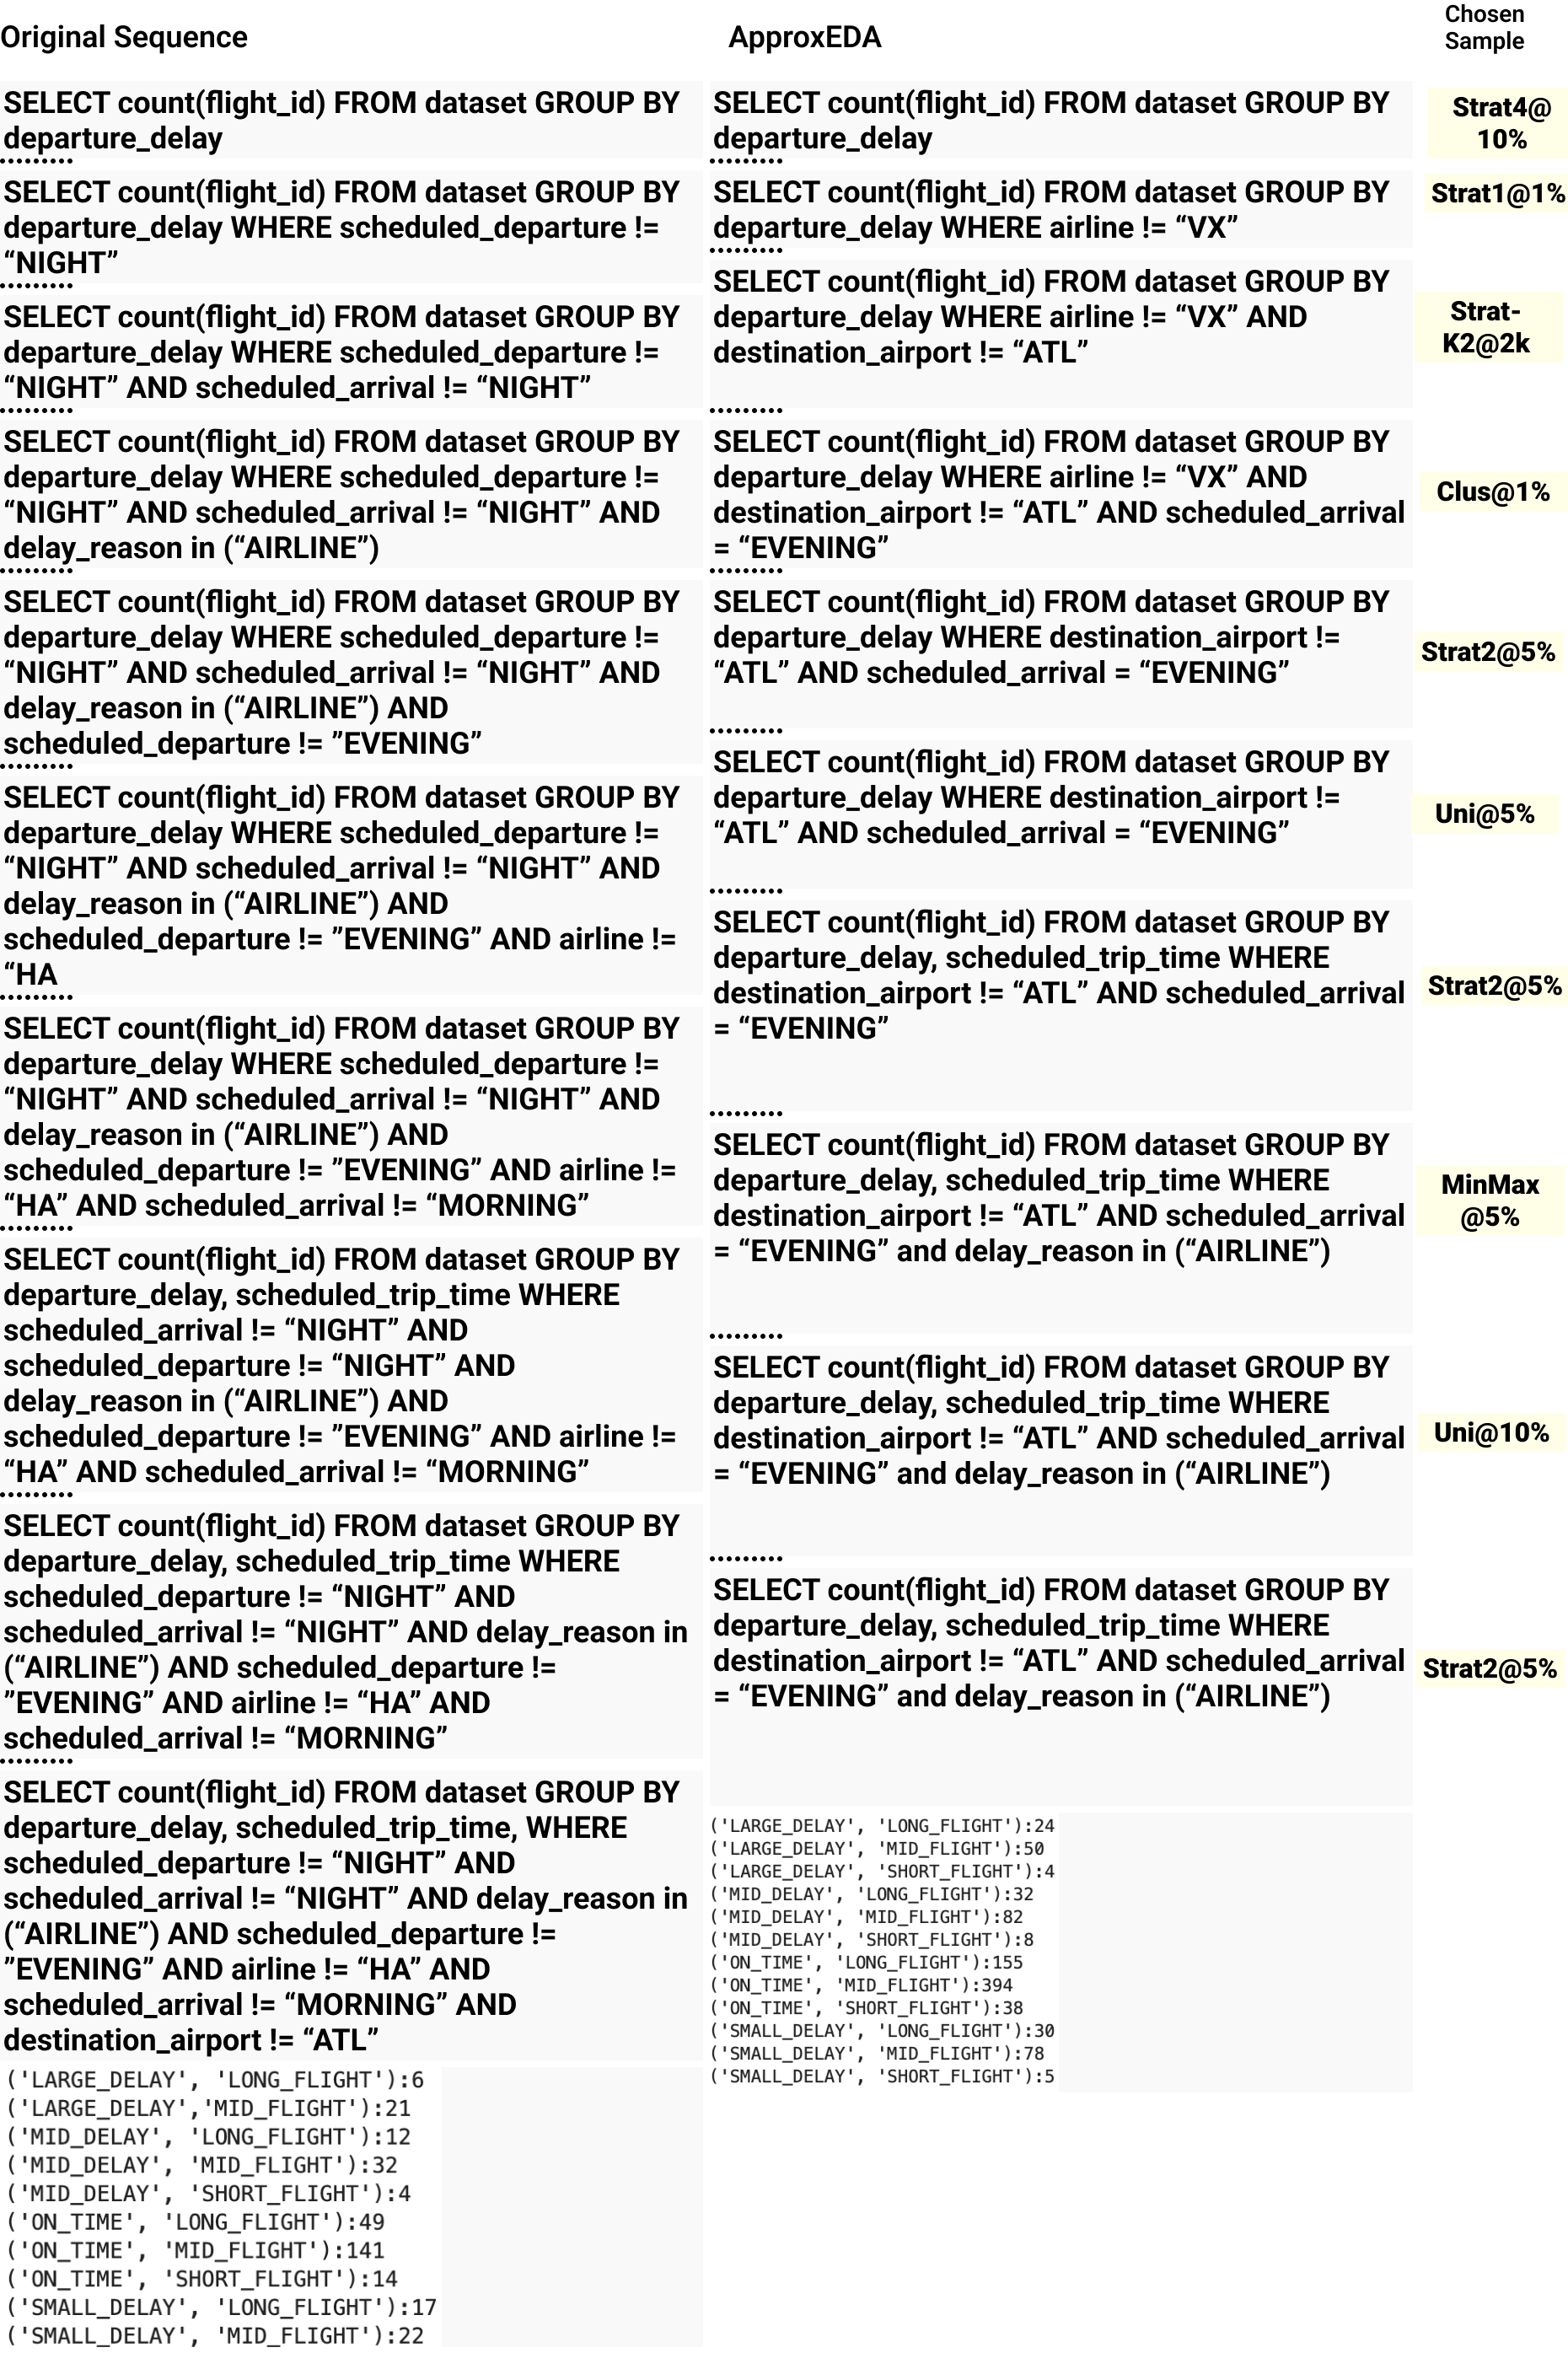
\includegraphics[width=1.0\columnwidth]{LaTeX/figures/appendix_seq.png}
     \caption{%Snapshot of an EDA sequence 
     An example EDA sequence from the logged results,
     showing how \name{} can efficiently preserve the query structure, analysis sequence and final outcome/insight by selecting various different samples (annotations on the right) under the hood to maximize its objective.}
     \label{fig:real}
\end{minipage}
\end{figure}

Figure~\ref{fig:real} we show a real EDA session with \name{}, where it 
selected various different samples (annotations on the right) to maximize its objective. We can see in-spite of it selecting fery frugal samples at various points (e.g. Clus@1\%, Uni@5\% etc.), \name{} can mostly preserve the query structure, analysis sequence and final outcome/insight. 
In Figure~\ref{fig:action_usage} we show the variation of \name{}'s choice of different actions (selection of samples) for 4 different intents identified for the Flights data across all the held out sequences.
We found that certain samples (e.g. MaxMin@5\%, Sys@20\%, Strat1@1\%) were predominantly chosen for certain intents (e.g. \#4). Intuition is that such samples can preserve representations of smaller groups better, which is necessary for that intent preservation.


%Then it will interact with the users' EDA sessions almost transparently. 


\subsection{Additional Results}
\label{app:add_res}
Similar to \ref{sec:eval_insight}, we also compute the recall for all the results instead of just 5. We show the results in \ref{fig:recall}. Even in the case of the whole recall \name{} seems to do better than the baselines.

\begin{figure}[!t]
\centering
\begin{minipage}[t]{0.495\columnwidth}
\vspace{0pt}
% \begin{table}[]
\scalebox{0.65}{
\begin{tabular}{|l|l|l|}
\hline
\begin{tabular}[c]{@{}l@{}}Sampling \\ Strategy\end{tabular} & \begin{tabular}[c]{@{}l@{}}No. of \\ Rows\end{tabular} & \begin{tabular}[c]{@{}l@{}}Effective\\  SR\end{tabular} \\ \hline
Uni@1\%                                                      & 5232                                                   & 0.01                                                    \\ \hline
Uni@5\%                                                      & 26155                                                  & 0.05                                                    \\ \hline
Uni@10\%                                                     & 52312                                                  & 0.1                                                     \\ \hline
Sys@100                                                      & 5231                                                   & 0.01                                                    \\ \hline
Sys@20                                                       & 26154                                                  & 0.05                                                    \\ \hline
Sys@10                                                       & 52311                                                  & 0.1                                                     \\ \hline
Clus@1\%                                                     & 5230                                                   & 0.01                                                    \\ \hline
Clus@5\%                                                     & 26154                                                  & 0.05                                                    \\ \hline
Clus@10\%                                                    & 52306                                                  & 0.1                                                     \\ \hline
MinMax@5\%                                                   & 27202                                                  & 0.052                                                   \\ \hline
MaxSum@5\%                                                   & 25109                                                  & 0.048                                                   \\ \hline
KStrat1@2k                                                   & 14124                                                  & 0.027                                                   \\ \hline
KStrat1@10k                                                  & 28771                                                  & 0.055                                                   \\ \hline
KStrat1@20k                                                  & 57542                                                  & 0.11                                                    \\ \hline
KStrat2@2k                                                   & 9416                                                   & 0.018                                                   \\ \hline
KStrat2@10k                                                  & 25125                                                  & 0.048                                                   \\ \hline
KStrat2@20k                                                  & 47080                                                  & 0.09                                                    \\ \hline
Strat1@1\%                                                   & 5220                                                   & 0.01                                                    \\ \hline
Strat1@5\%                                                   & 26146                                                  & 0.05                                                    \\ \hline
Strat1@10\%                                                  & 52375                                                  & 0.1                                                     \\ \hline
Strat2@1\%                                                   & 5232                                                   & 0.01                                                    \\ \hline
Strat2@5\%                                                   & 26148                                                  & 0.05                                                    \\ \hline
Strat2@10\%                                                  & 52320                                                  & 0.1                                                     \\ \hline
Strat3@1\%                                                   & 5240                                                   & 0.01                                                    \\ \hline
Strat3@5\%                                                   & 26150                                                  & 0.05                                                    \\ \hline
Strat3@10\%                                                  & 52315                                                  & 0.1                                                     \\ \hline
Strat4@1\%                                                   & 5235                                                   & 0.01                                                    \\ \hline
Strat4@5\%                                                   & 26149                                                  & 0.05                                                    \\ \hline
Strat4@10\%                                                  & 52321                                                  & 0.1                                                     \\ \hline
\end{tabular}
}
\captionof{table}{Details of Samples generated on Flights Dataset}
\label{tab:flights_samples}
\end{minipage}%
\hfill
\begin{minipage}[t]{0.495\columnwidth}
\vspace{0pt}
\begin{minipage}[t]{1.0\columnwidth}
\begin{minipage}[t]{1.0\columnwidth}
\vspace{0pt}
\scalebox{0.65}{
\begin{tabular}{|l|l|l|}
\hline
\begin{tabular}[c]{@{}l@{}}Sampling \\ Strategy\end{tabular} & \begin{tabular}[c]{@{}l@{}}No. of \\ Rows\end{tabular} & \begin{tabular}[c]{@{}l@{}}Effective\\  SR\end{tabular} \\ \hline
Uni@1\%                                                      & 3242                                                   & 0.01                                                    \\ \hline
Uni@5\%                                                      & 16210                                                  & 0.05                                                    \\ \hline
Uni@10\%                                                     & 32419                                                  & 0.1                                                     \\ \hline
Sys@100                                                      & 3241                                                   & 0.01                                                    \\ \hline
Sys@20                                                       & 16209                                                  & 0.05                                                    \\ \hline
Sys@10                                                       & 32419                                                  & 0.1                                                     \\ \hline
Strat1@1\%                                                   & 3246                                                   & 0.01                                                    \\ \hline
Strat1@5\%                                                   & 16225                                                  & 0.05                                                    \\ \hline
Strat1@10\%                                                  & 32425                                                  & 0.1                                                     \\ \hline
Strat2@1\%                                                   & 3238                                                   & 0.01                                                    \\ \hline
Strat2@5\%                                                   & 16215                                                  & 0.05                                                    \\ \hline
Strat2@10\%                                                  & 32426                                                  & 0.1                                                     \\ \hline
Strat3@1\%                                                   & 3240                                                   & 0.01                                                    \\ \hline
Strat3@5\%                                                   & 16208                                                  & 0.05                                                    \\ \hline
Strat3@10\%                                                  & 32420                                                  & 0.1                                                     \\ \hline
Strat4@1\%                                                   & 3248                                                   & 0.01                                                    \\ \hline
Strat4@5\%                                                   & 16206                                                  & 0.05                                                    \\ \hline
Strat4@10\%                                                  & 32425                                                  & 0.1                                                     \\ \hline
\end{tabular}
}

\captionof{table}{Details of Samples generated on Housing Dataset}
\label{tab:housing_samples}
\end{minipage}
\begin{minipage}[t]{1.0\columnwidth}
\scalebox{0.65}{
\begin{tabular}{|l|l|l|}
\hline
\begin{tabular}[c]{@{}l@{}}Sampling \\ Strategy\end{tabular} & \begin{tabular}[c]{@{}l@{}}No. of \\ Rows\end{tabular} & \begin{tabular}[c]{@{}l@{}}Effective\\  SR\end{tabular} \\ \hline
Uni@1\%                                                      & 4266                                                   & 0.01                                                    \\ \hline
Uni@5\%                                                      & 21334                                                  & 0.05                                                    \\ \hline
Uni@10\%                                                     & 42670                                                 & 0.1                                                     \\ \hline
Sys@100                                                      & 4266                                                  & 0.01                                                    \\ \hline
Sys@20                                                       & 21334                                                & 0.05                                                    \\ \hline
Sys@10                                                       & 42669                                                  & 0.1                                                     \\ \hline
Strat1@1\%                                                   & 4267                                                   & 0.01                                                    \\ \hline
Strat1@5\%                                                   & 21336                                                  & 0.05                                                    \\ \hline
Strat1@10\%                                                  & 42672                                                  & 0.1                                                     \\ \hline
Strat2@1\%                                                   & 4235                                                   & 0.01                                                    \\ \hline
Strat2@5\%                                                   & 21330                                                  & 0.05                                                    \\ \hline
Strat2@10\%                                                  & 42664                                                  & 0.1                                                     \\ \hline
Strat3@1\%                                                   & 4235                                                   & 0.01                                                    \\ \hline
Strat3@5\%                                                   & 21340                                                  & 0.05                                                    \\ \hline
Strat3@10\%                                                  & 42667                                                  & 0.1                                                     \\ \hline
Strat4@1\%                                                   & 4237                                                   & 0.01                                                    \\ \hline
Strat4@5\%                                                   & 21367                                                  & 0.05                                                    \\ \hline
Strat4@10\%                                                  & 42673                                                  & 0.1                                                     \\ \hline
\end{tabular}
}

\captionof{table}{Details of Samples generated on Income Dataset}
\label{tab:income_samples}
\end{minipage}
% \end{table}
\end{minipage}
\end{minipage}
\end{figure}


% \begin{figure*}[]
% \begin{minipage}[]{1\columnwidth}
% \begin{subfigure}{0.5\textwidth}
% 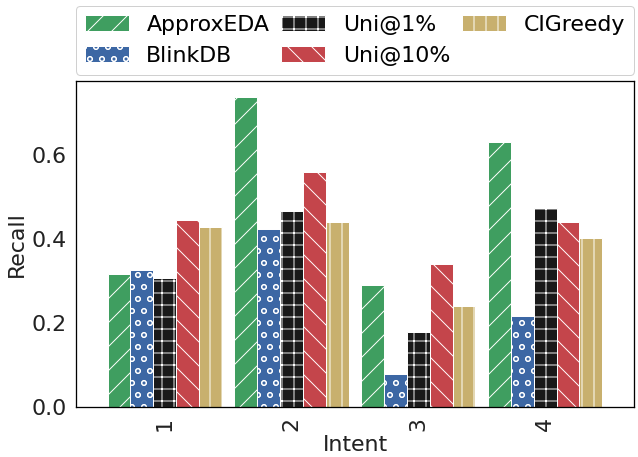
\includegraphics[width=1.0\linewidth]{LaTeX/figures/flights_eval1.png}
% \caption{Flights Dataset}
% \end{subfigure}
% \begin{subfigure}{0.5\textwidth}
% 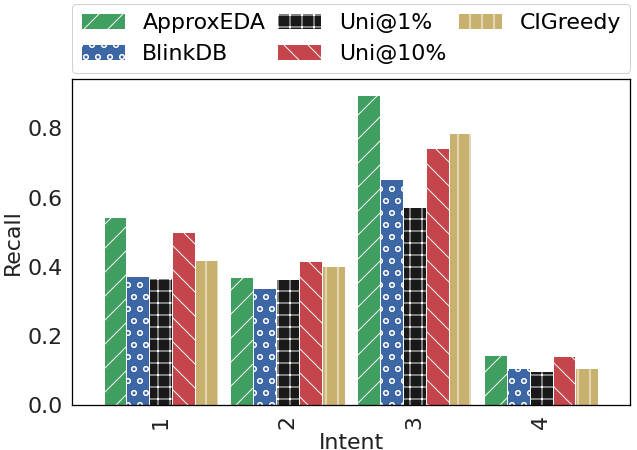
\includegraphics[width=1.0\linewidth]{LaTeX/figures/housing_eval1.png}
% \caption{Housing Dataset}
% \end{subfigure}
%      \caption{Insight Preservation: Recall of the resulting rows at the end of analysis sequence compared to results from full data, across various intents.
%      Higher is better.}
%      \label{fig:recall}
% \end{minipage}
% \end{figure*}


\subsection{Sampling Strategies}
\label{app:sampling_details}

A sample dataset $T_s$ is a subset of rows from an original dataset $T$. Following different sampling strategies select these subsets differently with different set of parameters that control the size and statistics of $T_s$.
%We now provide brief background for different sampling strategies we used. 

\noindent \textbf{Uniform Random Sampling:}
In uniform sampling, the rows of $T$ are
sampled independently (i.e, a Bernoulli process) with a sampling probability equal to $\tau \in [0,1] $. $\tau$ is called the sampling frequency and different values lead to different sizes for $T_s$.
%(and consequently different query latency).
%Total size of the sample:
%$|T_s| \approx \tau|T|$ (Note, Bernoulli process may not return exact number of rows as calculated using sampling probability).

\noindent \textbf{Systematic Sampling:}
In a systematic sample~\cite{lohr2019sampling}, a starting row of data is chosen using a random number. That row, and every $k$-th row thereafter, is chosen to be in $T_s$.
%With systematic sample thus $T_s$ consists of rows that are equally spaced in the data.
%Total size of the sample:
%$|T_s| = \floor*{{|T|}/{k}}$.
%If the rows are in random order, $T_s$ behaves much like an uniform random sample.
%However, systematic sampling does not necessarily give a representative sample when the rows are in some periodic or cyclical order. 
%Example, if male and female names alternate in a dataset, and $k$ is even, then
%$T_s$ will have either all men or all women data and can lead to wrong insights. 

\noindent \textbf{Stratified Sampling:}
Let for a column $C$ in data $T$, there are $G$ unique categories (i.e. strata). 
Stratified sample ensures that \textit{enough} rows are selected in $T_s$ for each unique values
%${v_1, \ldots , v_g}$ 
in $G$. 
%With $x$ denoting a row, let
%
%$T_i = \{x : x \in T \text{and $x$ takes values $v_i$ in column $C$}\}$

%Instead of doing such stratification for each column or all combination of columns,~\cite{agarwal2013blinkdb} proposed to use query column sets (QCS) that appear frequently as part of the filters (\texttt{WHERE}) and \texttt{GROUP BY} clauses in the query to reduce approximation error for ad-hoc queries.

%There are primarily two kinds of stratified samples used for query processing:
%\begin{itemize}
    %\item 
\noindent\textbf{Proportional stratified sample:} 
    In this case uniform samples $T_{i_{s}}$ are picked for each strata $T_{i}$ with a sampling probability of $\tau$.
    %Final sample $T_s = \bigcup\limits_{i=1}^{g} T_{i_{s}}$.
    %Different values of $\tau$ is selected to achieve approximation-latency trade-off.
    %Total size of the sample become: 
    
    %$|T_s| = \sum\limits_{i=1}^{g}{|T_{i_{s}}|} = \sum\limits_{i=1}^{g}{\tau|T_{i}|} $
    
    %\item 
\noindent\textbf{At most $K$ stratified sample:}
    In this case, for each strata, at most $K$ values are randomly selected to be included in $T_s$~\cite{agarwal2013blinkdb}.
    %Total size of the sample becomes: 
    
    %$|T_s| = \sum\limits_{i=1}^{g}\min(K, |T_{i}|)$
%\end{itemize}

\noindent \textbf{Cluster Sampling:}
The data is clustered into $k$  clusters,
%similar to stratified sampling, uniform 
samples are picked from each cluster with a sampling probability of $\tau$.
%Final sample $T_s = \bigcup\limits_{i=1}^{k} T_{i_{c}}$. %Total size of the sample becomes:

%$|T_s| = \sum\limits_{i=1}^{k}{|T_{i_{c}}|} = \sum\limits_{i=1}^{k}{\tau|T_{i}|} $
%Cluster has a superficial resemblance to strata: A cluster, like a stratum, is a
%grouping of the rows in $T$.
%However, when stratification generally increases precision when compared with simple random sampling, cluster sampling generally decreases it~\cite{lohr2019sampling}.

\noindent \textbf{Diversity sampling:} 
%Diversity sampling ensures that the algorithm picks out a diverse set of rows, $T_s$ from $T$. 
This targets that the sample picked out has different types of rows inside~\cite{diversity2017}. 
%Given a measure of diversity $div$, a set of rows $T$ having $|T|$ elements, and an integer $k$, $k < |T|$, we want to form a set $T_s$ containing $k$ elements of $T$, such that:
%
%$ T_s = \underset{T_s'  \subseteq T, |T_s'| = k}{\mathrm{argmax}}\, div(T_s') $
%
Diversity is defined by a distance function $d$, including: (i) \textbf{MaxMin Diversity:} 
    This maximises the minimum pairwise diversity between elements of $T_s$. 
    %We define the $div$ function as follows,
    %
    %$div(T_s') = \underset{i,j \in T_s', i \neq j}{\mathrm{min}}\, d(i,j) $
and (ii)  \textbf{MaxSum Diversity:}
    This maximises the average pairwise diversity between elements of $T_s$. 


Tables \ref{tab:flights_samples}, \ref{tab:housing_samples} and \ref{tab:income_samples} show the sampling strategies and corresponding parameters used, actual size of the samples ($|T_s|)$ and presents the Effective Sampling Rate (ESR) for each of the three datasets we used to evaluate. Lower the sample size, lower would be the query latency but at the cost of different magnitude of approximation errors depending on the actual sampling strategy. 

\begin{figure}[h]

    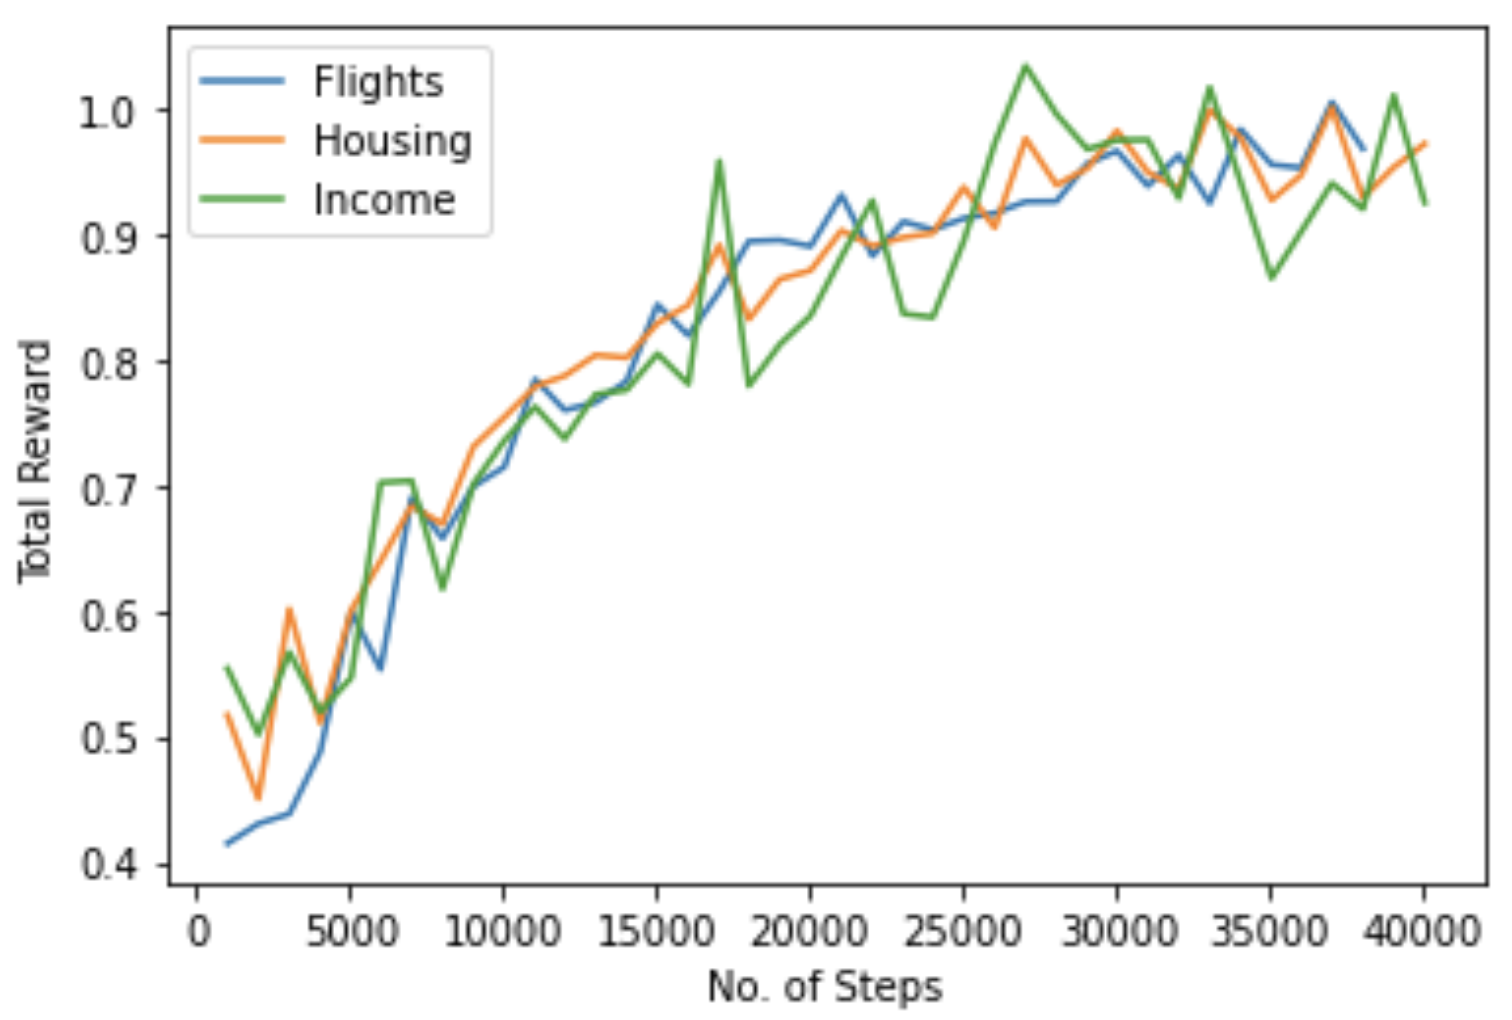
\includegraphics[width=1\linewidth]{LaTeX/figures/ss.png}
    \caption{RL training convergence curves for different datasets}
    \label{fig:my_conv}

\end{figure}
%\subsection{\name{} UI}
%
%In Figure~\ref{fig:demo} we show \name{}'s UI with which user will interact for EDA. The whole intelligence of \name{} remains almost transparent to the user. User can enable \name{} feature (blue box), to significantly improve interaction speed and \name{} will work at the background to choose optimal samples to run user-given query in an analysis flow and produce the results after each step. A log panel prints the actions taken by the RL-agent, along with corresponding query latency. Optionally, user can investigate the set of sampling strategies available. 
\end{document}
